\documentclass{article}

\usepackage{epsfig}
\usepackage[margin=1in]{geometry}
\usepackage[round]{natbib}
\usepackage{amsmath}
\usepackage{amsfonts}
\usepackage[capitalise]{cleveref}
\usepackage{verbatim}
\usepackage{float}
\usepackage{graphicx}
\usepackage{subcaption}


\newcommand{\bO}{\mathcal{O}}
\newcommand{\bR}{\mathbb{R}}
\newcommand{\ostu}{\operatorname{stu}}
\newcommand{\oref}{\operatorname{ref}}
\newcommand{\argmin}[1]{\underset{#1}{\operatorname{arg\;min}}\;}

\title{Computational Methods for Principle Component Analysis Applied to
  Genotype Data}
\date{}

\begin{document}

\maketitle

\begin{abstract}
    Population stratification (PS) is an important confounder
    for the association between genotypes and phenotypes.
    To adjust for PS,
    we need to accurately estimate the ancestral structure
    in the study samples.
    This can be done effectively
    by using principle component (PC) analysis
    to predict the PC scores of the study genotypes
    from a set of reference genotypes.
    There are two major existing methods for predicting PC scores:
    simple projection (SP) and augmentation-decomposition-transformation (ADP).
    However, when the reference size is large,
    the former is computationally efficient but inaccurate
    (PC scores shrinking toward zero),
    while the latter is accurate but computationally costly ($\bO[n^3]$).
    To solve these problems,
    we created the genoPCA software
    that implemented 
    the adjusted projection (AP) method to remove the bias in SP, and
    the online ADP (OADP) method to speed up ADP.
    We compared the accuracy and computational efficiency of these four methods
    by conducting a simulation study
    with the GGS software.
    We also used them to study the UKbiobank data by using the 1000Genomes data as the reference.
    We found that AP achieved the accuracy of ADP without adding much runtime,
    while OADP reduced the runtime of ADP by $x$-fold without losing accuracy.
    Furturmore, when studying a large number of samples
    from a narrower geographic area
    where the signal-to-noise ratio is low,
    AP and OADP performed reasonably well
    while SP frequently misclassified the populations
    and the runtime of ADP became impractical.
    
    
    
    
\end{abstract}

\section{Introduction}

Population stratification (PS) is an important confounder for the association between
genotypes and phenotypes \citep{price2006principal}.
To adjust for PS, we need to accurately estimate the ancestry structure in the study samples.
Principle component analysis (PCA) is a multivariate statistical method
which finds the direction of the maximum variability among the samples.
By aggregating information across all genetic markers,
PCA can accurately infer the ancestry structure \citep{reich2008principal}.
To adjust for PS,
PCA can be applied to study data to calculate the principle component (PC) scores,
which are regarded as variables of ancestry direction
and can be used as covariates to adjust for.
An alternative approach for doing PCA is
predicting the PC scores of the study samples
by using some reference genotyped samples with detailed ancestry information.
This prediction-based approach allows not only adjustment for PS
but also infererence of the ancestry memberships of the study samples. 

The standard way of predicting PC scores is to find the PC loadings of the reference samples and project the study samples onto them.
We call this method simple projection (SP).
However, when the number of features greatly exceeds the size of the reference samples,
which is common for genotype data,
the PC scores predicted by SP are known to be biased toward null \citep{dey2016asymptotic}.
One way of addressing this shrinkage bias is presented by \citet{wang2014ancestry, wang2015improved}.
Their solution is to combine one study sample with all the reference samples and
find the PC scores of this augmented data set by using singular value decomposition (SVD).
The PC scores of the study individuals are then retrieved from the singular vector matrices and mapped to the reference PC space by a Procrustes transformation.
We call this method ``augmentation, decomposition, and Procrustes transformation'' (ADP).
This method has been shown to be effective in eliminating the shrinkage bias of study PC scores.
However since ADP needs to run SVD for each study sample,
ADP is computationally expensive.

To address the limitations of SP and ADP,
we propose and evaluate two alternative PC score prediction methods.
The first approach removes the bias in SP by estimating the asymptotic bias factor,
which is calculated based on random matrix theory \citep{dey2016asymptotic}.
The second approach improves the computational efficiency of ADP
by using an online SVD algorithm \citep{halko2011finding}, 
which obtains the SVD results of the augmented matrix
by updating the SVD results of the reference matrix,
since the latter only differs slightly from the former
and the overlapping calculations can be avoided
(at least approximately).
We call the first approach ``adjusted projection'' (AP)
and the second approach ``online augmentation, decomposition, and Procrustes transformation'' (OADP). 
We found that AP and OADP have both achieved accuracy close to that of ADP
and computational efficiency close to that of SP.

\section{Method}

\subsection{Model}

\subsubsection{Data Format}
For PC score prediction,
we have a reference group and a study group.
The reference and study data sets are represented by matrices.
Let $X$ be a $p \times n$ matrix of reference genotypes
and  let $Y$ be a $p \times m$ matrix of study sample genotypes,
where $p$ is the number of genetic markers,
$n$ is the number of reference samples
and $m$ is the number of study samples.
In our study we only consider genotypes composed of biallelic single nucleotide polymorphisms (SNP),
so each entry of $X$ and $Y$ is a minor allele count of 0, 1, or 2.

\subsubsection{Principle Component Analysis on the Reference Data}
First, we conduct a PCA on the reference data $X$.
The reference data matrix is standardized
so that the mean and standard deviation of each feature are $0$ and $1$, respectively.
With $n$ data points residing in a $p$-dimensional vector space and $n < p$,
there is a unique $n$-dimensional hyperplane that covers all the data points.
This hyperplane can be represented as the span of an orthonormal basis composed of $n$ unit vectors.
Of course, the choice for such orthonormal basis is not unique,
but what what we are interested in PCA is 
to maximize the variance of the samples on the direction of the first basis element,
maximize the variance on the samples on the second basis element after they are collapsed in the direction of the first basis element,
and so forth,
until we have $n$ basis elements.
At the end, PCA gives us three variables:
\begin{enumerate}
    \item $n$ pairwise-orthogonal unit vectors of $p$ dimensions
    representing the orthonormal basis.
    These are called principle components (PC) or PC loadings,
    and we organized them into a $p \times n$ matrix $U$.
    \item $n$ non-negative real numbers
    each of which represents the standard deviations of the samples
    on the direction of the corresponding PC loading.
    They are organized into an $n \times n$ diagonal matrix $D$.
    \item $n$ tuples of $n$ dimensions
    representing the normalized coordinates of the data points
    in the $n$-dimensional space spanned by the PC loadings.
    These are called the normalized PC scores,
    and they are organized into an $n \times n$ matrix $V$,
    where each column corresponds to the coordinate of a PC loading
    and each row corresponds to a sample.
\end{enumerate}
If we multiply each normalized PC score by the corresponding standard deviation
(i.e. calculate $VD$),
we get the unnormalized PC scores.
In our study, we use unnormalized PC scores and simply call them PC scores.
The study can be carried out by using normalized PC scores, too,
and the result would be equivalent.
Moreover, the standard deviation matrix $D$ is in descending order,
so that the first column of $U$ is the direction of the greatest sample variance,
the first column of $V$ represents the coordinates of the $n$ samples in this direction.
The same correspondence applies to $U$'s and $V$'s second column, third column, etc.
Thus PCA reduces the dimension of the sample space from $p$ to $n$.
We can further reduces the sample space dimension
by using only the first $k$ PCs ($k \ll n$) and ignore the rest $n-k$ PCs.
In genetic studies, choosing $k \leq 10$ is often sufficient.

The (standardized) reference data matrix can be restored by $X = U D V^T$.
In fact, this is exactly the SVD of $X$ \citep{jolliffe2002principal}.
Thus PCA on the reference data can be done easily on any language
in which a SVD algorithm has been implemented.
If all that we are interested in is the PC scores,
we can reduce the computational complexity by applying eigen decomposition (EGD) on $X^TX$
to obtain $X^T X = V D^2 V^T$.
Afterwards, $U$ can be retrieved by $U = X V D^{-1}$ if needed.

\subsubsection{Predicting the PC Scores of the Study Samples}

Once PCA is finished on the reference data,
we predict the PC scores of the study data.
There are more than one ways to accomplish this,
and two common methods are SP and ADP.
The performance of these two methods can be improved by using AP and OADP.
We now discuss the algorithm, computational efficiency, and accuracy of these four methods.

Before we using any of these methods,
we need to standardize the study samples
by subtracting the reference means from them
and then dividing them by the reference standard deviations.
For simplicity,
we overload the symbol $Y$
and let it represent the standardized study data for the rest of the paper.

\paragraph{Simple Projection (SP)}
This method is simple and intuitive.
Since the PCA on the reference data has already given us the PC loadings,
we can simply project a (standardized) study sample onto them by calculating their dot products.
The resulted projection lengths are the predicted PC scores for this study sample.
The algorithm is

\begin{enumerate}
\item Compute the reference covariance matrix $X^T X$.
  (Computational complexity (CC): $\bO[pn^2]$.)  
\item EGD on the reference covariance matrix: $X^T X = V D^2 V^T$.
  (CC: $\bO[n^3]$.)
\item Compute the PC loading matrix for the top $k$ PCs only: $U_k= X V_k D_k^{-1}$.
Here $V_k$ and $D_k$
are the the first $k$ columns of $V$
and the upper-left $k \times k$ submatrix of $D$, respectively.
(CC: $\bO[pnk]$.)
\item Compute the predicted study PC scores for the top $k$ PCs: $W_k = Y^T U_k$.
(CC: $\bO[mpk]$.)
\end{enumerate}
The total computational complexity is  $\bO[pn^2 + mpk]$
given that $k \ll n \ll p$.
The computational complexity for each study sample is $\bO[pk]$,
which is the lowest among all the methods discussed in this paper.
However, though computationally efficient,
a major disadvantae of SP is the loss of accuracy when the number of features $p$ greatly exceeds the reference sample size $n$,
a situation that is not uncommon for genotype data.
\citet{dey2016asymptotic} have shown that when $n \ll p$,
especially when the signals in the reference samples are not strong,
the predicted PC scores will shrink toward the origin.
This shrinkage bias limits the accuracy of SP for high dimensional data.
Fortunately, \citet{dey2016asymptotic} have also provided a way
to estimate the asymptotic shrinkage magnitude and angle
and implemented it in the \verb|hdpca| package in the R language \citep{hdpca}.
We use this estimation to eliminate the shrinkage bias,
as in the AP method.

\paragraph{Adjusted Projection (AP)}

This method is almost identical to SP,
with the only difference being the addition of the adjustment for the shrinkage bias
after the projections are finished to restore the unshrinked PC scores.
For estimating the asymptotic shrinkage factor,
we need all the eigenvalues
of the the reference data matrix,
as well as the number of features
and the reference sample size.
The details for estimating the shrinkage factor can be found in \citet{dey2016asymptotic}.
The algorithm is summarized below.

\begin{enumerate}
\item Compute the reference covariance matrix $X^T X$.
  (CC: $\bO[pn^2]$.)  
\item EGD on the reference covariance matrix: $X^T X = V D^2 V^T$.
  (CC: $\bO[n^3]$.)
\item Estimate the shrinkage magnitudes and organize them in a $n \times n$ diagonal matrix $S$.
  (CC: $\bO[p]$.)
\item Compute the PC loading matrix for the top $k$ PCs with the adjustment for the shrinkage bias: $U_k= X V_k D_k^{-1} S_k^{-1}$.
Here $V_k$, $D_k$, and $S_k$
are the the first $k$ columns of $V$
and the upper-left $k \times k$ submatrices $D$ and $S$, respectively.
(CC: $\bO[pnk]$.)
\item Compute the predicted study PC scores for the top $k$ PCs: $W_k = Y^T U_k$.
(CC: $\bO[mpk]$.)
\end{enumerate}
Given that $k \ll n \ll p$,
the total computational complexity is $\bO[pn^2 + mpk]$,
which is the same as that of SP.
Thus the adjustment for the shrinkage bias in AP
does not increase the computational complexity of SP
(though it does slightly increase the empirical runtimes).
A minor disadvantage of AP is that
while the computatinal complexity and memory usage of SP
can be further reduced
by using some truncated SVD algorithm
(such as the randomized SVD algorithm
by \citet{halko2011finding}
as discussed in \cref{sec:randsvd})
to compute the SVD for only the top $k$ PCs of the reference matrix,
AP requires all the eigenvalues
and thus a full SVD or EGD of the reference matrix.

\paragraph{Augmentation, Decomposition, and Procrustes Transformation (ADP)}

ADP predicts the study PC scores by using a completely different approach
compared to SP and AP.
The details of this method
and an implementation in C++ called TRACE
are described in \cite{wang2014ancestry,wang2015improved}.
In ADP,
we augment the (standardized) reference matrix by one column
by appending a (standardized) study sample to it.
Then we apply SVD or EGD to this $p \times (n+1)$ matrix $\tilde{X}$.
The resulted $(n+1) \times (n+1)$ normalized PC score matrix $\tilde{V}$
can be divided into two submatrices:
the first $n$ rows $\tilde{V}_{\oref}$,
which correspond to the reference samples,
and the last row $\tilde{v}_{\ostu}$,
which corresponds to the study sample.
Notice that $\tilde{V}_{\oref}$ is now different from $V$,
the $n \times n$ normalized PC score matrix of the reference data,
so we look for a linear transformation
\[
    f(\tilde{V}_{\oref}) = \rho A \tilde{V}_{\oref} + c
\]
where $\rho$ is a non-negative real number
(for uniform scaling),
$A$ is a $n \times (n+1)$ orthonormal matrix
(for projection, rotation and reflection),
and $c$ is a column vector
(for translation),
so that the distance
between $V$ and the transformed $f(\tilde{V}_{\oref})$
(i.e. the sum of squares of the error matrix $V - f(\tilde{V}_{\oref})$)
is minimized.
This is called the Procrustes transformation
from $f(\tilde{V}_{\oref})$ to $V$.
We then apply this transformation to $\tilde{v}_{\ostu}$
to obtain $f(\tilde{v}_{\ostu})$.
Finally,
by multiplying these Procrustes-transformed normalized PC scores
by the reference PC standard deviations,
we obtain the predicted PC score for the study sample $f(\tilde{v}_{\ostu})D$.

Notice that so far we have been using all the PCs for ADP.
However, this is not necessary
if all that we are interested in
is the top few PCs.
Thus we can use only
the top $k$ PC scores of the reference matrix
and the top $lk$ PC scores of the augmented matrix
(where $l$ is a constant greater than or equal to $1$ and $lk \ll n$)
and find the Procrustes transformation from $\bR^{lk}$ to $\bR^k$.
The algorithm is summarized as follows.

\begin{enumerate}
\item Compute the reference covariance matrix $X^T X$.
  (CC: $\bO[pn^2]$.)  
\item Apply EGD to the reference corariance matrix
  to obtain $X^T X = V D^2 V^T$.
  (CC: $\bO[n^3]$.)
\item For a study sample $y$,
  find the augmented covariance matrix
  $\tilde{X}^T \tilde{X}$
  by computing $X^T y$, $(X^T y)^T$, and $y^T y$
  and appending them to the
  bottom edge,
  right edge,
  and bottom-right corner of $X^TX$.
  (CC: $\bO[pn]$.)
\item Apply EGD to $\tilde{X}^T \tilde{X}$ to get $\tilde{X}^T \tilde{X} = \tilde{V} \tilde{D}^2 \tilde{V}^T$.
  (CC: $\bO[n^3]$.)
\item Find the Procrutes transformation
from the first $lk$ columns of $\tilde{V}$
to the first $k$ columns of $V$.
  (CC: $\bO[nk^2]$)
  \item Go to step 3 for the next study sample
  until all the study samples are analyzed.
\end{enumerate}
The total computational complexity is
$\bO[pn^2 + m(np + n^3)]$
given that $lk \ll n \ll p$.

ADP is regarded as the most accurate method for predicting study PC scores.
It is does not have SP's shrinkage bias.
However, the major disadvantage of ADP
is its high computational complexity.
In particular,
as the reference size increases,
the computational cost for a study sample
increases cubically.
Fortunately, this disadvantage can be mitigated by taking some computational shortcuts,
as in the OADP method.

\paragraph{Online Augmentation, Decomposition, and Procrustes Transformation (OADP)}

Notice that the augmented data matrix $\tilde{X}$
only differs slightly from the reference matrix $X$
when the reference sample size is large.
Thus the computational process for the SVD of $\tilde{X}$
is numerically close to that for the SVD of $X$.
If we can avoid the repeated computation in this process
and obtain the SVD of $\tilde{X}$
by updating the SVD of $X$
instead of recalculating everything,
we could greatly reduce the computational cost.
One of such ``online'' algorithms for computing the SVD of the augmented matrix is discussed in \citet{brand2002incremental}.
This algorithm calculates SVD in the incremental manner described above
and has the ability to find the approximate SVD for the top few singular values only,
which exactly fits our need for obtaining the top few PCs.
Thus we use the algorithm by \citet{brand2002incremental}
to replace the standard algorithm for decomposing the augmented matrices
and coin the name ``online augmentation, decomposition, and Procrustes transformation'' (OADP).
The algorithm for this method is as follows:

\begin{enumerate}
\item Compute $X^T X$.
  (Computational complexity: $\bO[n^2p]$.)  
\item Apply eigendecomposition to $X^T X$ to get $X^T X = V D^2 V^T$.
  ($\bO[n^3]$.)
\item Calculate $U_3 = X V_3 D_3^{-1}$,
  where $V_3$ is the first $k_3$ columns of $V$,
  and $D_3$ is the diagonal matrix of the first $k_3$ diagonal entries of $D$.
  ($\bO[k_3 n p]$.)
\item Calculate 
  \[
    L = U_3^T y \quad \text{and} \quad K = y^T H,
  \]
  where $H$ is the normalized  $y - U_3L$
  ($\bO[k_3 p]$.)
\item Calculate $Q^T Q$, where
  \[
    Q = 
    \begin{bmatrix}
      D_3 & L \\
      0 & K
    \end{bmatrix}.
  \]
  ($\bO[k_3^3]$.)
\item Apply eigendecomosition to $Q^T Q$ to get $Q^T Q = \ddot{V}_3 \ddot{D}^2_3 \ddot{V}^T_3$.
  ($\bO[k_3^3]$.)
\item Calculate
  \[
    \tilde{V}_3 =
    \begin{bmatrix}
      V_3 & 0 \\
      0 & 1
    \end{bmatrix}
    \ddot{V}_3.
  \]
  ($\bO[nk_3^2]$.)
\item Project the first $k_2$ columns of $\tilde{V}_3$ to the first $k_1$ columns of $V$ by using Procrustes analysis to get the transformed PC scores of the study individual,
  where $k_1 < k_2  < k_3 \ll n$.
  (Computational complexity is ignorable if $k_2$ is not large compared to $n$.)
  \item Go to step 4 for the next study individual.
\end{enumerate}

Total computational complexity: $\bO[n^2p + n^3 + k_3np + m(k_3p + k_3^3 + nk_3^2]) \approx \bO[n^2p + m(k_3p + k_3^2n)]$, provided $k_3 \ll n \ll p$.

The computational complexity of OADP for the study individuals increases linearly with respect to the reference sample size, which makes the computation time of OADP close to those of SP.
The closeness between the results given by OADP and ADP will be empirically shown later.

A comparison of computational complexities of the four PCA methods are shown in \Cref{tbl:cplx}.

\subsection{Simulation Studies}

We used the Grid Genotype Simulator (GGS)
by \citet{ mathieson2012differential}
to simulate population migration.
The grid's dimension is 2 by 2
with the same number of individuals
in each of the 4 populations.
Moreover, we let the number of reference samples
range from 1000 to 3000
and fix the number of study samples to 200.
Each genotype sample has 100 genealogies
with 1000 loci in each genealogy.
In addition, the migration rate was set to 100.
After the individuals were simulated,
we applied SP, ADP, AP, and OADP to the data
to predict the PC scores for the study samples.
Then we used the k-nearest neighbors method
to predict which ethnic group a study sample comes from.

\subsection{UK Biobank data analysis}

We also applied the four methods
to study the UK Biobank data \citep{sudlow2015uk},
which consists of 490,000 middle- or elderly-aged individuals
in the United Kingdom.
Our reference samples
are from the 1000 Genomes Project \citep{10002015global},
which collected 2500 samples from Europe, Africa, East Asia, South Asia, and America.
(Individuals whose children are also in the data were removed.)
The reference and the study samples
have 145,000 SNPs in common.
After we predicted the PC scores and ethnic groups
of the study samples,
we selected the study samples predicted to by Europeans
and applied PCA to them
by using the European reference samples only.
Since ADP is very slow compared to the other three methods,
we randomly selected 500 study samples
and used them to compare the four methods.
After that,
we applied SP, AP, and OADP to all the study samples.


\section{Results}

\subsection{Simulation study}

% Runtimes vs ref size
% Distance to ADP vs ref size
% Distance to geo center vs ref size
% PC1 vs PC2, 5 x 3 grid (uncolored study samples)
% The predicted PC scores are shown in \Cref{fig:n1000} and \Cref{fig:ukb}.

For the simulation study,
the PC scores predicted by AP, OADP, and ADP
are very close to each other
for every choice of reference sample size.
Compared to their results,
SP exhibits a strong shrinkage
when the reference sample size is 1000.
As we gradually increases the reference sample size to 3000
by an increment of 500,
the magnitude of the shrinkage decreases
but is still visible.
This is consistent with the theoretical result
that the shrinkage bias decreases
as the ratio of
the reference sample dimension to the reference sample size
decreases \citep{dey2016asymptotic}.

For computational cost,
we can see that the runtime for SP increases faster than linearly
as the reference sample size increases.
This is consistent
with the theoretical computational complexity of SP,
which expects the runtime to increase at the rate of $\bO[n^3]$.
In comparison, the runtimes of SP, AP, and OADP
increase only slightly.
The theoretical computational complexity of SP and AP is $\bO[1]$
and that of OADP is $\bO[n]$,
when the data dimension and the study sample size are fixed.

\subsection{UK Biobank data}

When we used the global samples in the UK Biobank data,
we found that the PC scores predicted by the four methods' are almost identical.
The separation of the ethnic groups was clear,
and the shrinkage bias of SP was not obvious,
which is consistent with the theoretical understanding
that the shrinkage bias decreases
as the signal-to-noise ratio increases.

However, when we focused on the European (EUR) samples only,
the results given by SP were clearly unreliable.
The samples from British in England and Scotland (GBR)
and those from Utah residents with northern and western European ancestry	(CEU)
drifted very close to NULL.
This causes SP to incorrectly classified almost all of them as CEU,
since most GBR reference samples are far away from NULL.
A few of the study samples predicted by ADP to be GBR or CEU
were even classified as the Iberian population in Spain (IBS),
since the IBS reference samples are close to NULL.
Moreover, the shrinkage for the IBS
and for the Toscani in Italia (TSI) populations
caused significant errors within these two groups.
The IBS reference samples
are approximately in the middle
between the TSI reference samples and NULL.
Thus most of the the study samples predicted by ADP to be TSI
were classified by SP as IBS.

For OADP, its predicted PC1 and PC2 scores
for the European study samples
are almost identical
to those done by ADP.
OADP's results for PC3 and PC4
are also very close to ADP's results,
though we observed a very slight decrease in the magnitude of the PC scores.
This minor shrinkage did not affect
OADP's classification for the IBS and TSI samples,
since their PC1 and PC2 scores were accurately predicted by OADP.
Neither was any CEU/GBR sample classified as IBS/TSI. 
For the CEU and GBR samples,
their predicted PC scores are tightly mixed together
for all the 4 PCs,
which were even difficult for ADP to separate them.
Thus the slight difference in PC3 and PC4 scores
between OADP and ADP
caused the classification of many CEU and GBR samples
to be different on the two methods.

Furthermore, AP successfully adjusted for the shrinkage
in PC1 and PC2 for the European samples,
so its predicted PC scores are almost identical to ADP's.
However, it did not detect the shrinkage in PC 3 and PC4,
so its predicted PC scores are the same as SP's for these two PCs.
This still allowed AP to correctly separate
the CEU/GBR samples from the IBS/TSI samples.
However, its separation of the IBS and TSI samples
did not agree completely with that done by ADP,
most likely caused by the shrinkage on PC3.
For the classification between CEU and GBR,
the AP's results differ far from ADP's,
as AP classified many more CEU/GBR samples as CEU.

The patterns for the accuracy of SP, AP, and OADP
discussed above
were also observed
when we used all the 490,000 study samples in the UK Biobank dataset
and those predicted to be Europeans among them.
See \Cref{tbl:ukb} for details.


\section{Discussion}

For the future, we would like
to improve the parallelization of our software.
Currently it uses the poor-man’s parallelism,
that is,
dividing the study dataset into multiple smaller files on the hard drive,
applying the analysis to each of them,
and merge the results.
This parallelism saves both the memory usage and the runtime.
However, we would like to utilize
more sophisticated parallel computation techniques
to further improve the performance of our software.

\newpage

\appendix
\bibliographystyle{plainnat}
\bibliography{paper}

\newpage
\section{Tables and Figures}

\begin{figure}[p]
\begin{subfigure}{.5\textwidth}
  \centering
  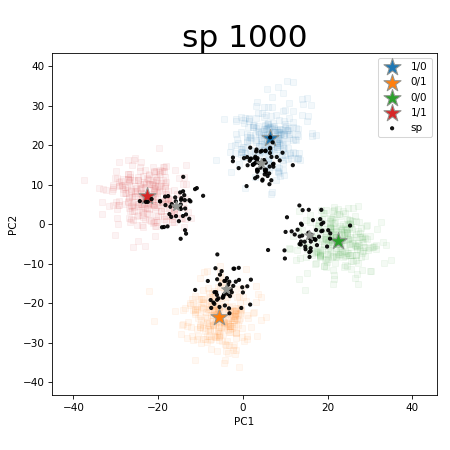
\includegraphics[width=.98\linewidth]{img/ggsim1000_100000_200_2_1_100_1_sturef_ggsim1000_100000_1000_2_1_100_0_sp}
\end{subfigure}%
\begin{subfigure}{.5\textwidth}
  \centering
  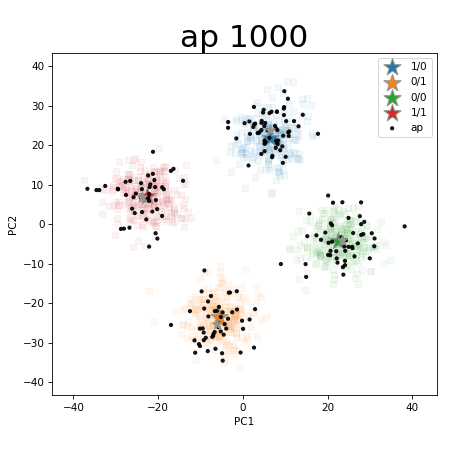
\includegraphics[width=.98\linewidth]{img/ggsim1000_100000_200_2_1_100_1_sturef_ggsim1000_100000_1000_2_1_100_0_ap}
\end{subfigure}
\hfill
\begin{subfigure}{.5\textwidth}
  \centering
  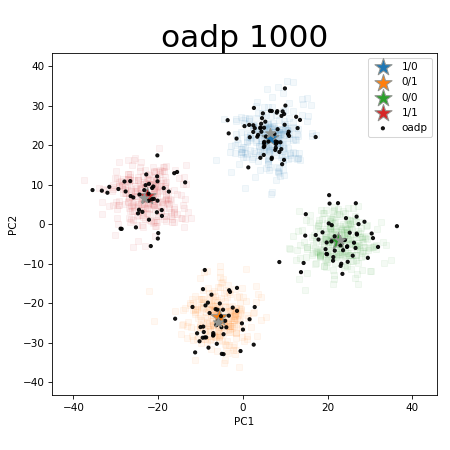
\includegraphics[width=.98\linewidth]{img/ggsim1000_100000_200_2_1_100_1_sturef_ggsim1000_100000_1000_2_1_100_0_oadp}
\end{subfigure}%
\begin{subfigure}{.5\textwidth}
  \centering
  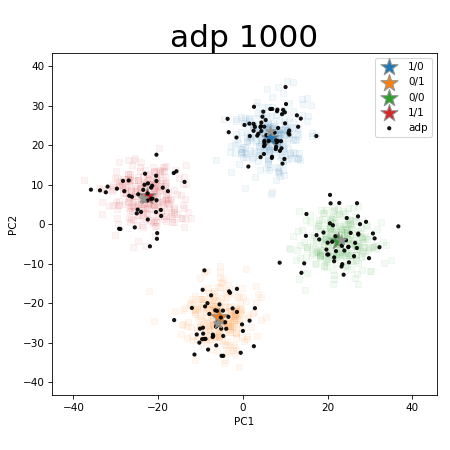
\includegraphics[width=.98\linewidth]{img/ggsim1000_100000_200_2_1_100_1_sturef_ggsim1000_100000_1000_2_1_100_0_adp}
\end{subfigure}
\end{figure}

\begin{figure}[p]
\begin{subfigure}{.5\textwidth}
  \centering
  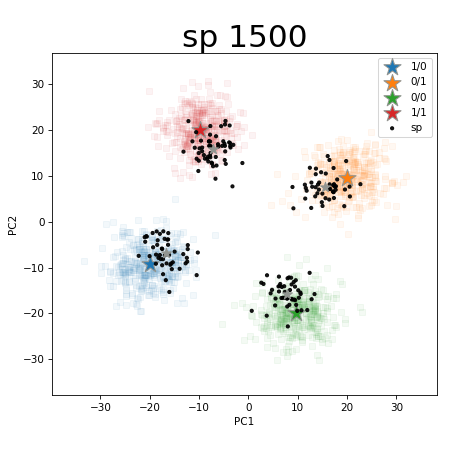
\includegraphics[width=.98\linewidth]{img/ggsim1500_100000_200_2_1_100_1_sturef_ggsim1500_100000_1500_2_1_100_0_sp}
\end{subfigure}%
\begin{subfigure}{.5\textwidth}
  \centering
  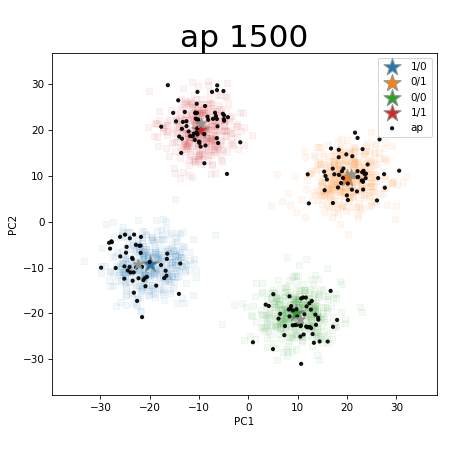
\includegraphics[width=.98\linewidth]{img/ggsim1500_100000_200_2_1_100_1_sturef_ggsim1500_100000_1500_2_1_100_0_ap}
\end{subfigure}
\hfill
\begin{subfigure}{.5\textwidth}
  \centering
  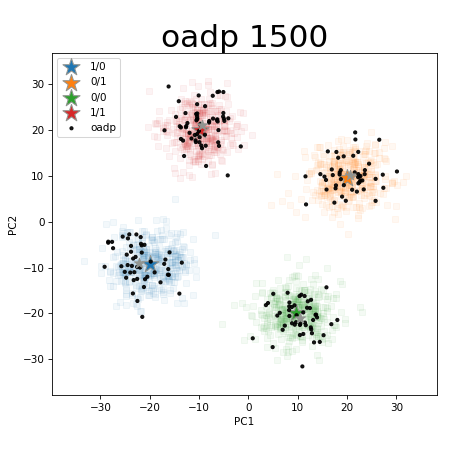
\includegraphics[width=.98\linewidth]{img/ggsim1500_100000_200_2_1_100_1_sturef_ggsim1500_100000_1500_2_1_100_0_oadp}
\end{subfigure}%
\begin{subfigure}{.5\textwidth}
  \centering
  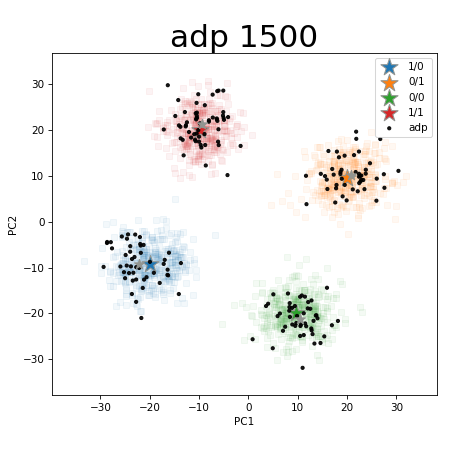
\includegraphics[width=.98\linewidth]{img/ggsim1500_100000_200_2_1_100_1_sturef_ggsim1500_100000_1500_2_1_100_0_adp}
\end{subfigure}
\end{figure}

\begin{figure}[p]
\begin{subfigure}{.5\textwidth}
  \centering
  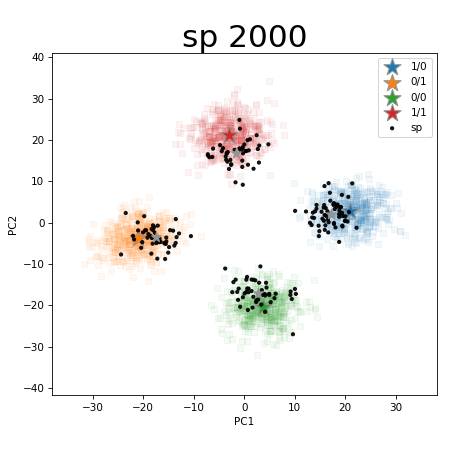
\includegraphics[width=.98\linewidth]{img/ggsim2000_100000_200_2_1_100_1_sturef_ggsim2000_100000_2000_2_1_100_0_sp}
\end{subfigure}%
\begin{subfigure}{.5\textwidth}
  \centering
  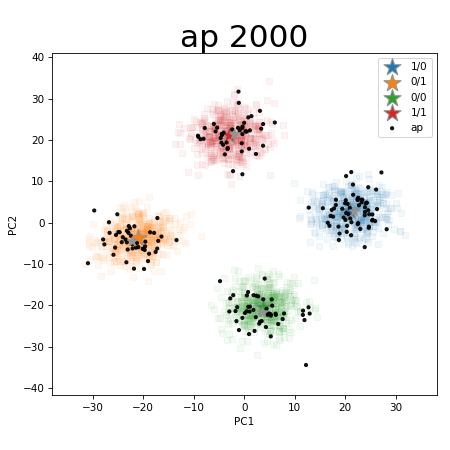
\includegraphics[width=.98\linewidth]{img/ggsim2000_100000_200_2_1_100_1_sturef_ggsim2000_100000_2000_2_1_100_0_ap}
\end{subfigure}
\hfill
\begin{subfigure}{.5\textwidth}
  \centering
  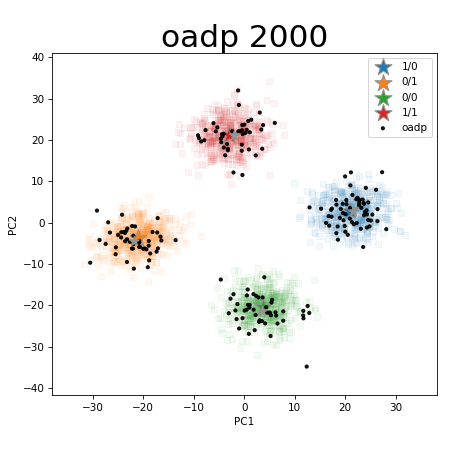
\includegraphics[width=.98\linewidth]{img/ggsim2000_100000_200_2_1_100_1_sturef_ggsim2000_100000_2000_2_1_100_0_oadp}
\end{subfigure}%
\begin{subfigure}{.5\textwidth}
  \centering
  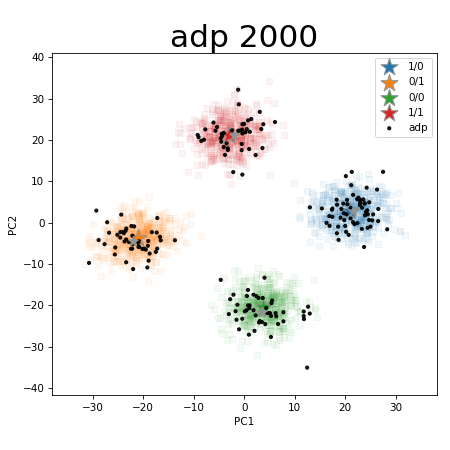
\includegraphics[width=.98\linewidth]{img/ggsim2000_100000_200_2_1_100_1_sturef_ggsim2000_100000_2000_2_1_100_0_adp}
\end{subfigure}
\end{figure}

\begin{figure}
\begin{subfigure}{.5\textwidth}
  \centering
  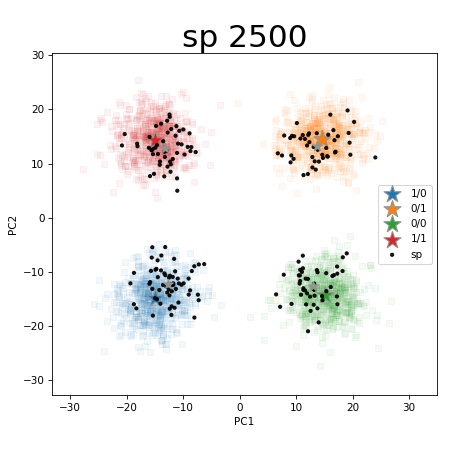
\includegraphics[width=.98\linewidth]{img/ggsim2500_100000_200_2_1_100_1_sturef_ggsim2500_100000_2500_2_1_100_0_sp}
\end{subfigure}%
\begin{subfigure}{.5\textwidth}
  \centering
  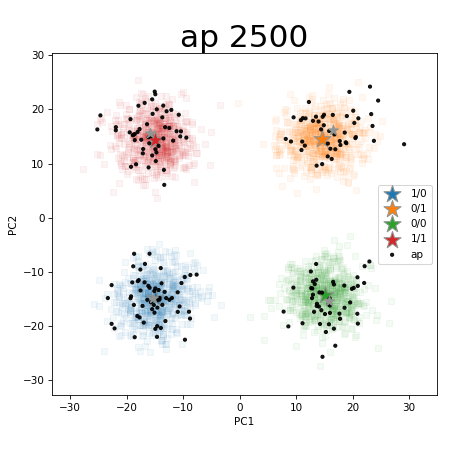
\includegraphics[width=.98\linewidth]{img/ggsim2500_100000_200_2_1_100_1_sturef_ggsim2500_100000_2500_2_1_100_0_ap}
\end{subfigure}
\hfill
\begin{subfigure}{.5\textwidth}
  \centering
  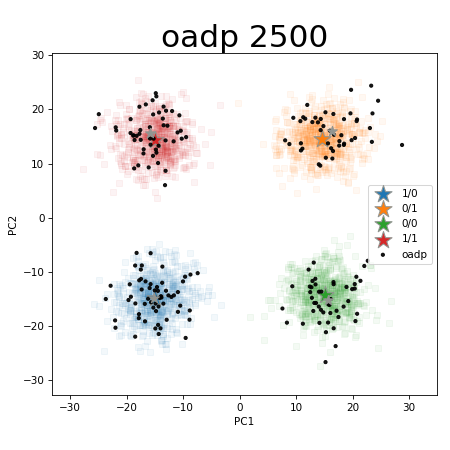
\includegraphics[width=.98\linewidth]{img/ggsim2500_100000_200_2_1_100_1_sturef_ggsim2500_100000_2500_2_1_100_0_oadp}
\end{subfigure}%
\begin{subfigure}{.5\textwidth}
  \centering
  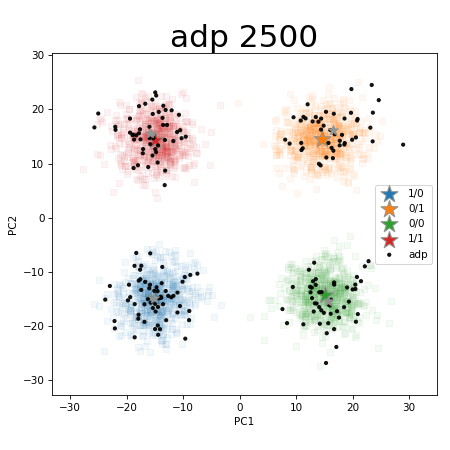
\includegraphics[width=.98\linewidth]{img/ggsim2500_100000_200_2_1_100_1_sturef_ggsim2500_100000_2500_2_1_100_0_adp}
\end{subfigure}
\end{figure}

\begin{figure}
\begin{subfigure}{.5\textwidth}
  \centering
  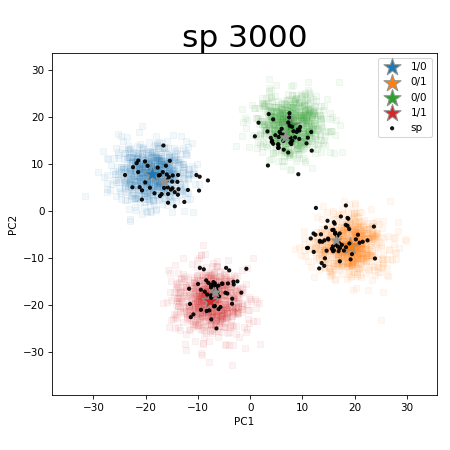
\includegraphics[width=.98\linewidth]{img/ggsim3000_100000_200_2_1_100_1_sturef_ggsim3000_100000_3000_2_1_100_0_sp}
\end{subfigure}%
\begin{subfigure}{.5\textwidth}
  \centering
  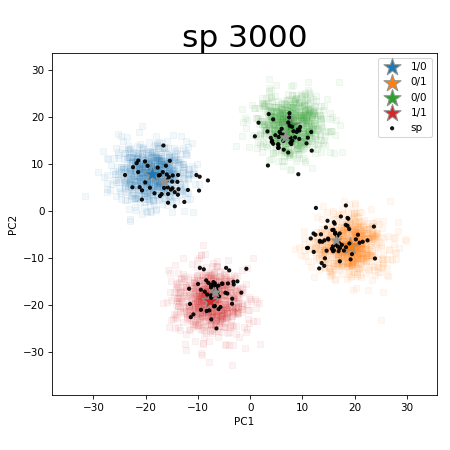
\includegraphics[width=.98\linewidth]{img/ggsim3000_100000_200_2_1_100_1_sturef_ggsim3000_100000_3000_2_1_100_0_sp}
\end{subfigure}
\hfill
\begin{subfigure}{.5\textwidth}
  \centering
  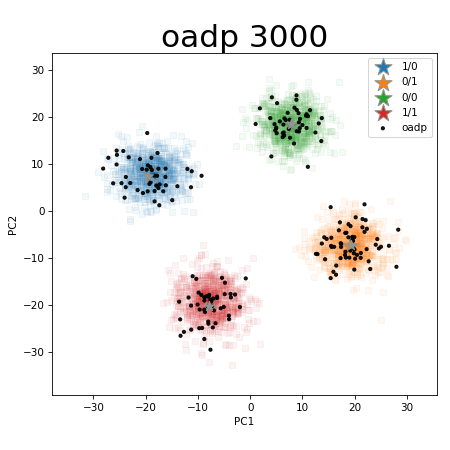
\includegraphics[width=.98\linewidth]{img/ggsim3000_100000_200_2_1_100_1_sturef_ggsim3000_100000_3000_2_1_100_0_oadp}
\end{subfigure}%
\begin{subfigure}{.5\textwidth}
  \centering
  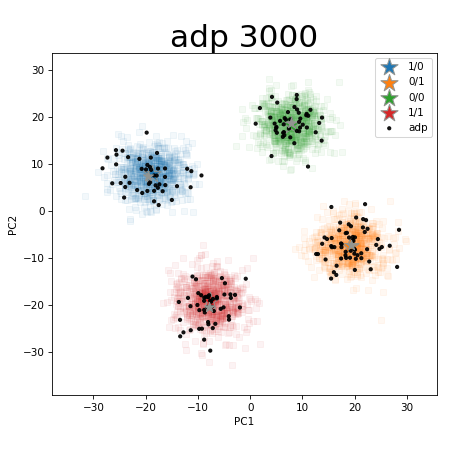
\includegraphics[width=.98\linewidth]{img/ggsim3000_100000_200_2_1_100_1_sturef_ggsim3000_100000_3000_2_1_100_0_adp}
\end{subfigure}
\caption{
  The PC scores predicted by each of the four methods
  as the reference size varies.
  Reference samples are in colors
  and study samples are in black.
  The stars mark the centers of mass (geographic centers) of each population for the reference and study samples.
  The number of variants is 100,000,
  and the study sample size is 200.
  Only the top 4 PCs are calculated.
  The data is simulated by the GGS software \citep{mathieson2012differential}.
}
\end{figure}

\begin{table}[h]
  \centering
  \begin{tabular}{|l|l|l|}
    \hline
    Method & Reference Complexity & Study Complexity \\ 
    \hline
    ADP & $\bO[n^2 p]$ & $\bO[mn(p + n^2)]$ \\
    \hline
    OADP & $\bO[n^2 p]$ & $\bO[mk(p + k n)]$ \\
    \hline
    SP & $\bO[n^2p]$ & $\bO[mkp]$ \\
    \hline
    AP & $\bO[n^2p]$ &  $\bO[mkp]$ \\
    \hline
  \end{tabular}
  \caption{
    Comparison of computational complexity for different methods.
    Here $p$ is the number of SNPs,
    $n$ is the number of individuals in the reference group,
    $m$ is the number of individuals in the  study group,
    and $k$ is the number of PCs calculated by the corresponding method.
  }
  \label{tbl:cplx}
\end{table}

\begin{table}[h]
  \centering
  \begin{tabular}{|l|l|l|l|l|l|}
    \hline
    Reference Size & 1000 & 1500 & 2000 & 2500 & 3000 \\
    \hline
    \multicolumn{6}{|c|}{Study Runtime} \\
    \hline
    SP         &  17  & 17   & 16   & 18   & 18   \\
    AP         &  18  & 16   & 18  & 16   & 17  \\
    OADP       &  145  & 146   & 147   & 148   & 149   \\
    ADP        &  379  & 809 & 1526 & 2556 & 4062 \\
    \hline
    \multicolumn{6}{|c|}{Distance from ADP's results} \\
    \hline
    SP         &  188  & 139   & 112   & 91   & 84   \\
    AP         &  31  & 27   & 12  & 11   & 14  \\
    OADP       &  21  & 16   & 12   & 9   & 10   \\
    ADP        &  0  & 0 & 0 & 0 & 0 \\
    \hline
    \multicolumn{6}{|c|}{Distance from reference centers} \\
    \hline
    SP         &  335 & 161  & 113 & 71  & 60  \\
    AP         &  31  & 19   & 17  & 25  & 15  \\
    OADP       &  12  & 17   & 11  & 20  & 12  \\
    ADP        &  20  & 14   & 14  & 23  & 14  \\
    \hline
  \end{tabular}
  \caption{
    The runtimes and errors of the four methods
    as the reference size increases.
    Distances are measured by the Euclidean distance.
    Reference centers are the centers of mass of the populations
    in the reference samples.
    The number of variants is 100,000,
    and the study sample size is 200.
    Only the top 4 PCs are calculated.
    The data is simulated by the GGS software \citep{mathieson2012differential}.
    }
\end{table}

\begin{figure}[h]
  \centering
  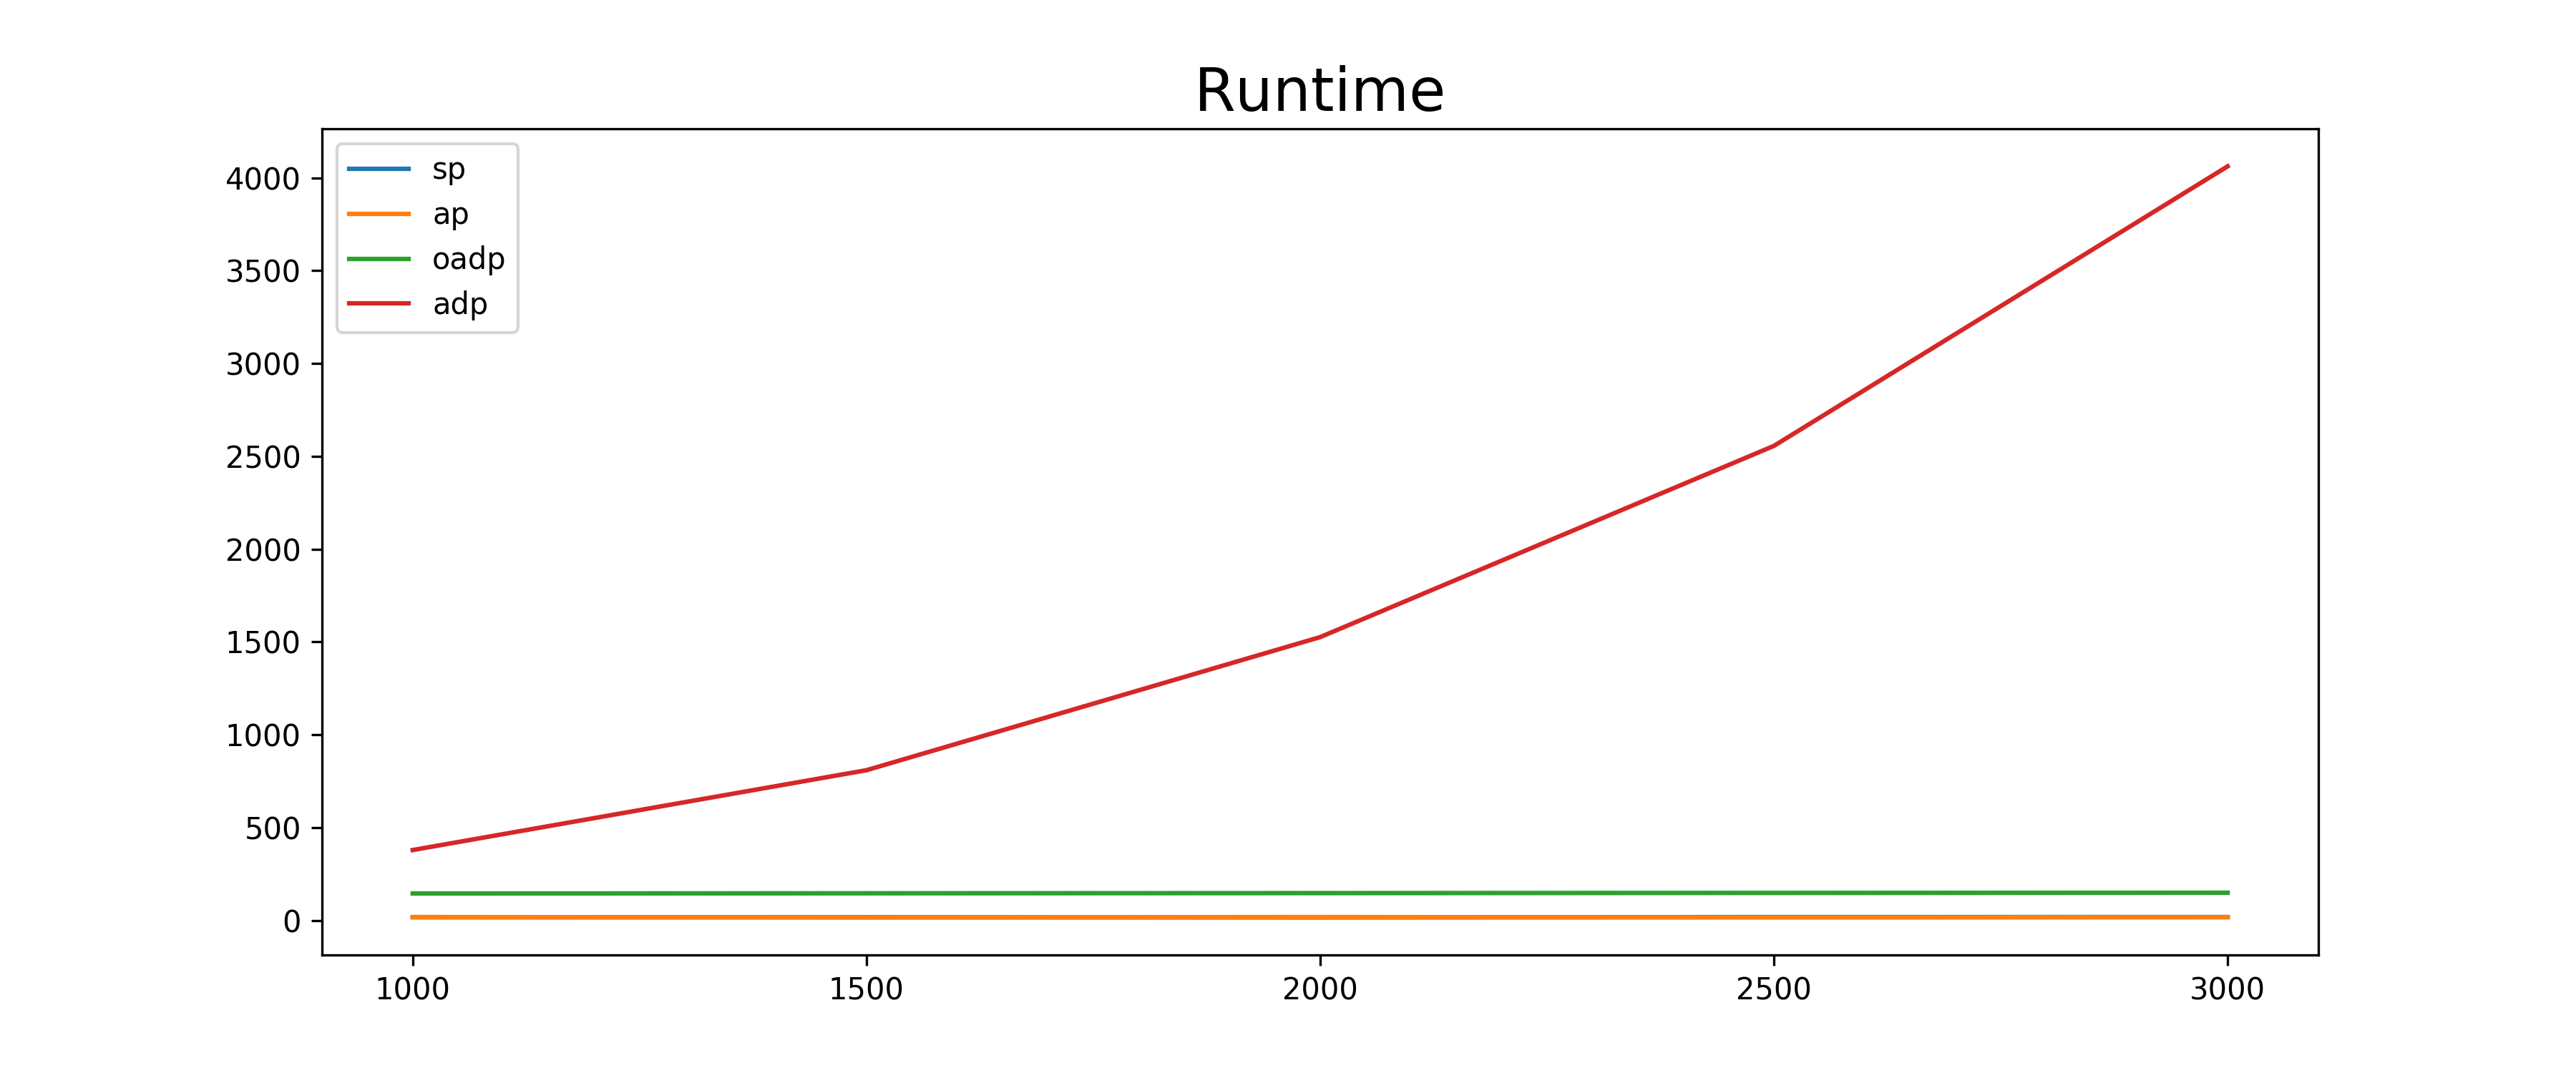
\includegraphics[width=.98\linewidth]{img/ggsim_runtimes.png}
  \centering
  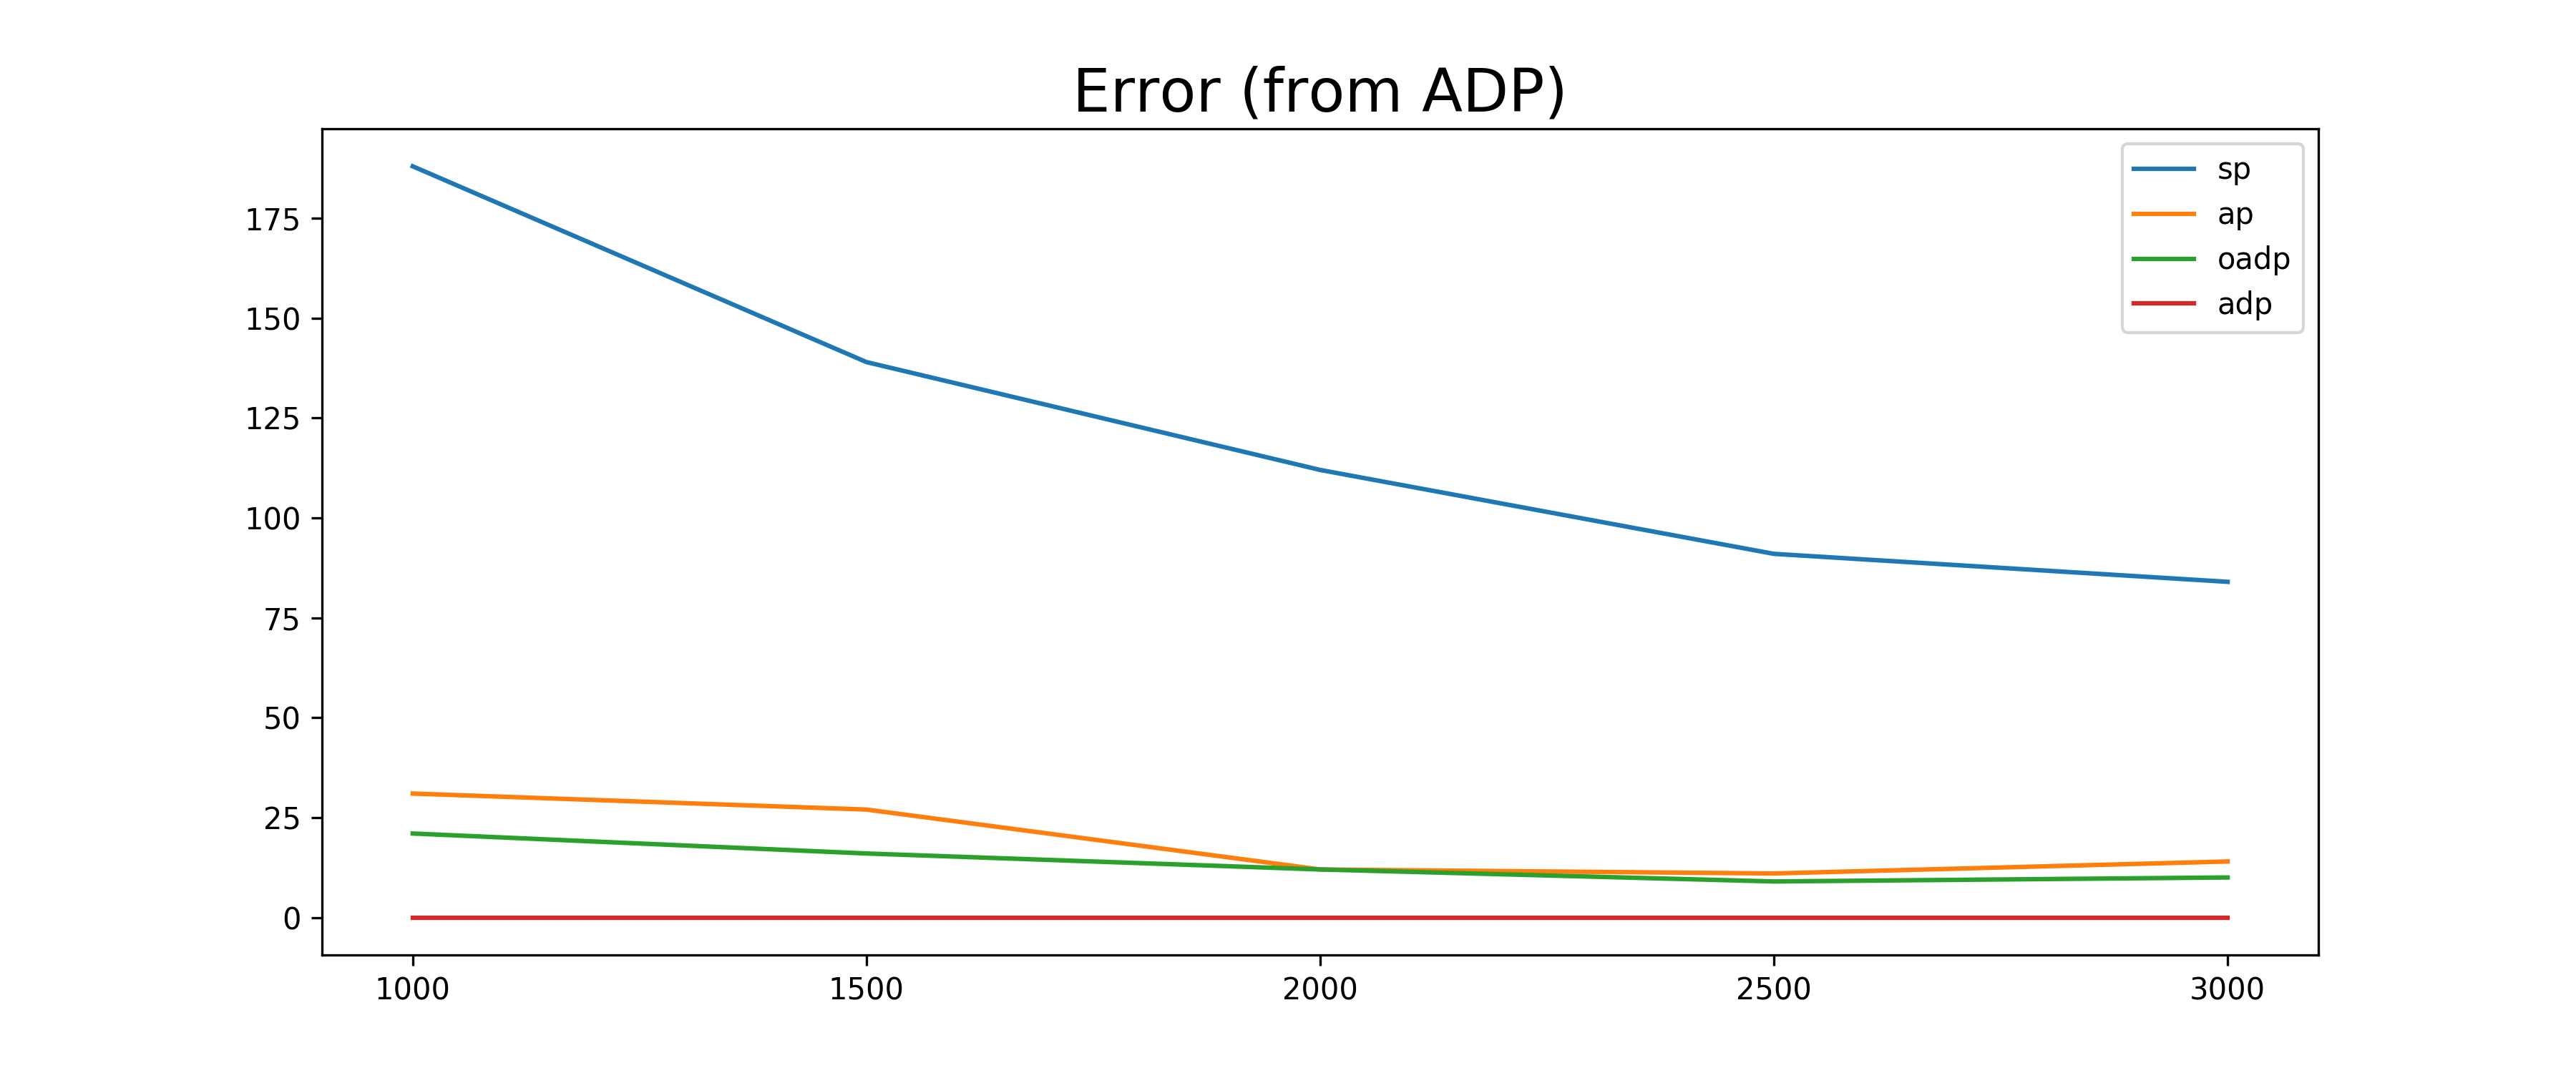
\includegraphics[width=.98\linewidth]{img/ggsim_errors_adp.png}
  \centering
  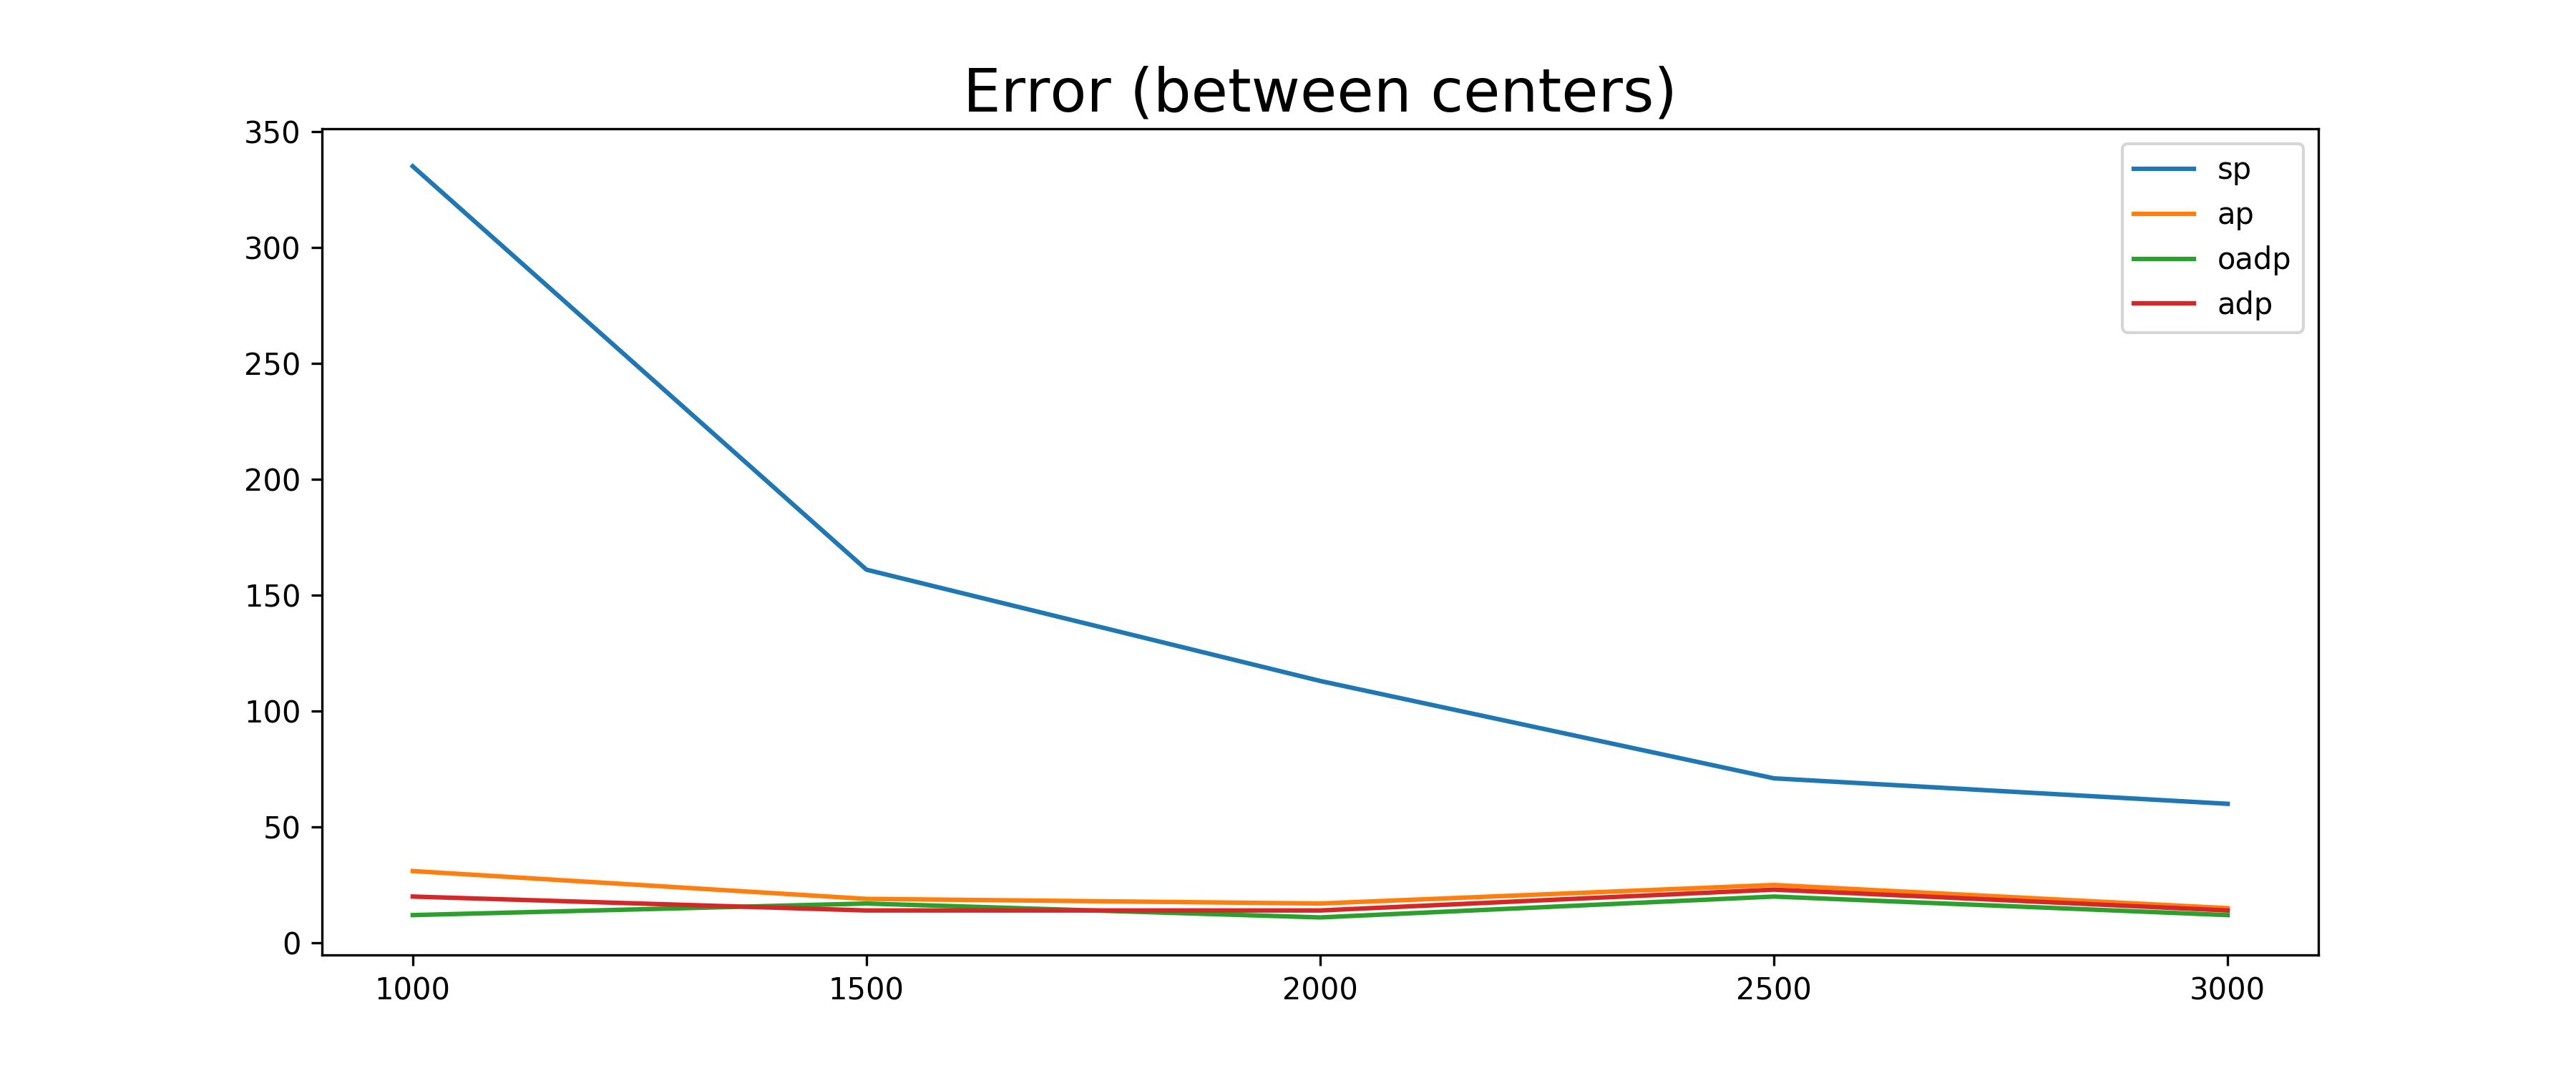
\includegraphics[width=.98\linewidth]{img/ggsim_errors_ctr.png}
  \caption{
    The runtimes and errors of the four methods
    as the reference size increases.
    Runtimes are measured in seconds.
    Errors from ADP are the Euclidean distance
    from each method's result to ADP's result.
    Errors between centers are the Euclidean distance
    from the centers of mass of the reference populations
    to the corresponding centers of mass of the study populations.
    The number of variants is 100,000,
    and the study sample size is 200.
    Only the top 4 PCs are calculated.
    The data is simulated by the GGS software \citep{mathieson2012differential}.
  }
\end{figure}

\begin{table}[H]
  \centering
  \begin{tabular}{|r|r|r|r|r|r|r|}
    \hline
    Method & \multicolumn{2}{|c|}{Runtime} & \multicolumn{2}{|c|}{Error (ADP)} & \multicolumn{2}{|c|}{Error (centers)} \\
    \hline
    & Global & European & Global & European & Global & European \\
    \hline
    SP         &  62   & 48  & 92  & 450 & 3156 & 2304 \\ 
    AP         &  65   & 48  & 48  & 33  & 2486 & 706  \\
    OADP       &  363  & 349 & 10  & 32  & 2575 & 665  \\
    ADP        &  6739 & 518 & 0   & 0   & 2578 & 649  \\
    \hline
  \end{tabular}
  \caption{
    The study runtimes (in seconds) and erros for the four methods
    for 500 randomly selected study samples
    in the UK Biobank data.
    Errors (ADP) are the Euclidean distances from
    the PC scores predicted by each method
    to those predicted by ADP.
    Errors (centers) are the Euclidean distances
    from the centers of mass of the reference samples
    to the centers of mass of the study samples.
    For the global study,
    2492 samples from the 1000 Genomes data are used as the reference.
    For the European study,
    only the 498 European samples among them are used.
    The number of variants in common is 145,282.
    Only the top 4 PCs are calculated.
    }
\end{table}

\begin{figure}[p]
  \centering
  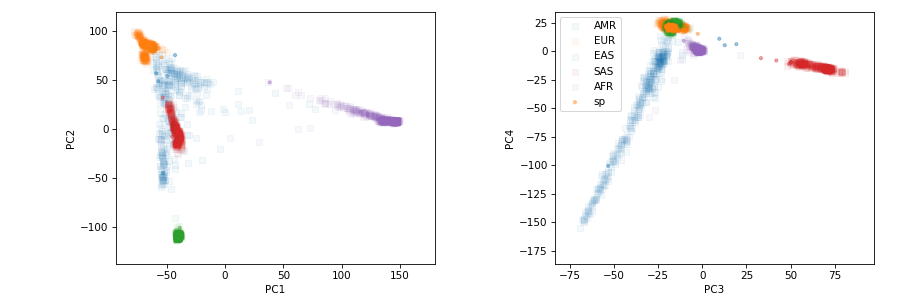
\includegraphics[width=0.98\textwidth]{img/ukb_snpscap_kgn_bial_orphans_5c_sturef_kgn_bial_orphans_snps_ukb_snpscap_ukb_sp}
  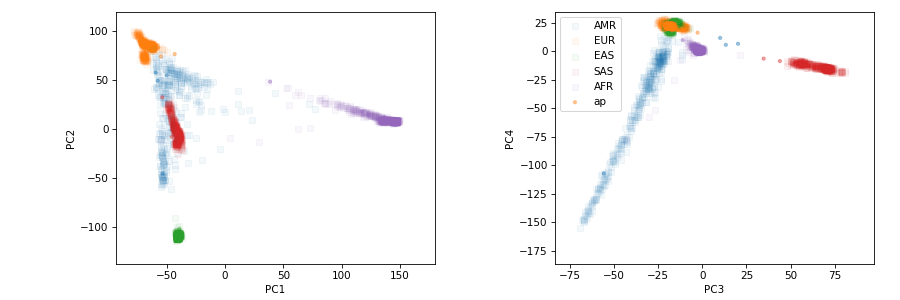
\includegraphics[width=0.98\textwidth]{img/ukb_snpscap_kgn_bial_orphans_5c_sturef_kgn_bial_orphans_snps_ukb_snpscap_ukb_ap}
  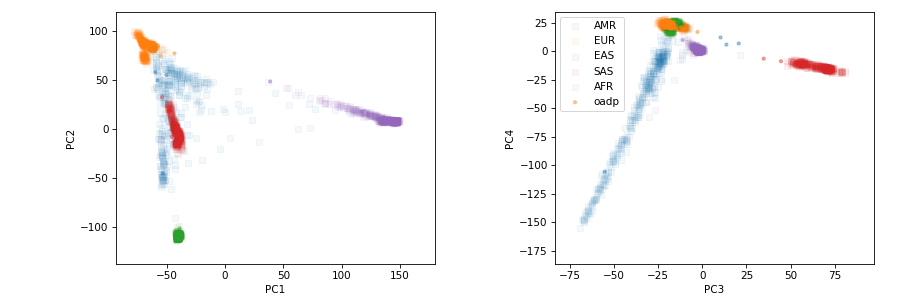
\includegraphics[width=0.98\textwidth]{img/ukb_snpscap_kgn_bial_orphans_5c_sturef_kgn_bial_orphans_snps_ukb_snpscap_ukb_oadp}
  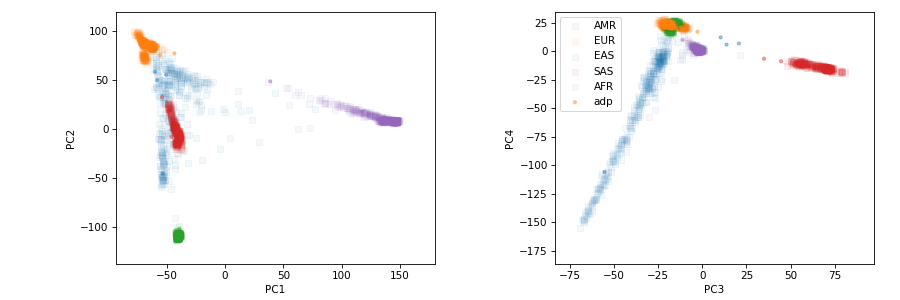
\includegraphics[width=0.98\textwidth]{img/ukb_snpscap_kgn_bial_orphans_5c_sturef_kgn_bial_orphans_snps_ukb_snpscap_ukb_adp}
  \caption{PC scores of 500 randomly selected global samples in UK Biobank data (circles) predicted by the four methods with the global samples in the 1000 Genomes data (squares) as the reference.}
\end{figure}

\begin{figure}[p]
  \centering
  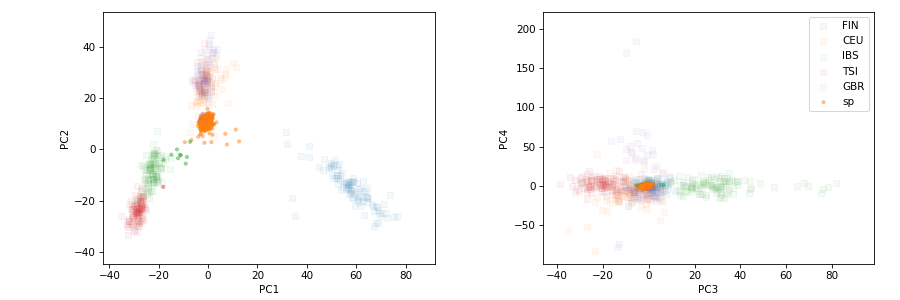
\includegraphics[width=0.98\textwidth]{img/ukb_snpscap_kgn_bial_orphans_5c_pred_EUR_sturef_kgn_bial_orphans_snps_ukb_snpscap_ukb_EUR_sp}
  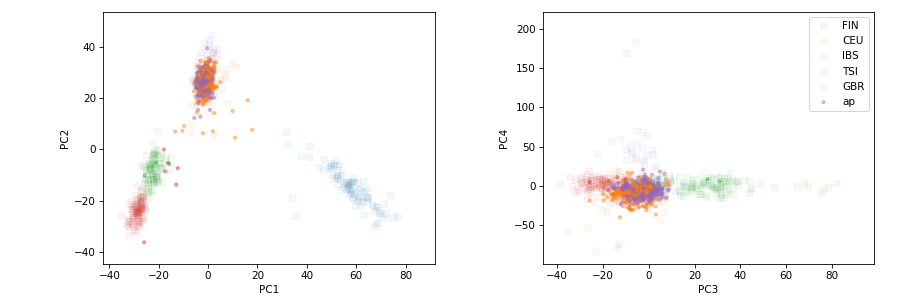
\includegraphics[width=0.98\textwidth]{img/ukb_snpscap_kgn_bial_orphans_5c_pred_EUR_sturef_kgn_bial_orphans_snps_ukb_snpscap_ukb_EUR_ap}
  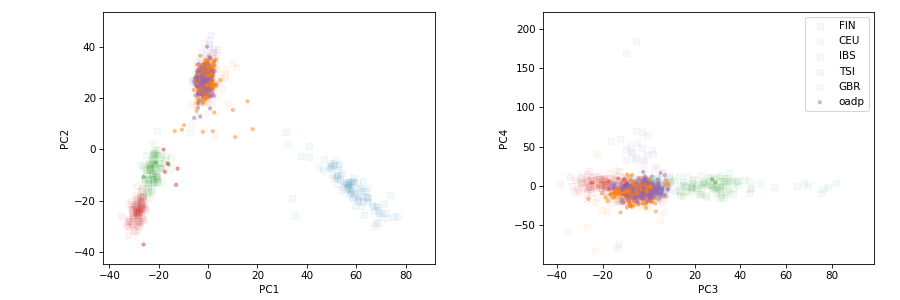
\includegraphics[width=0.98\textwidth]{img/ukb_snpscap_kgn_bial_orphans_5c_pred_EUR_sturef_kgn_bial_orphans_snps_ukb_snpscap_ukb_EUR_oadp}
  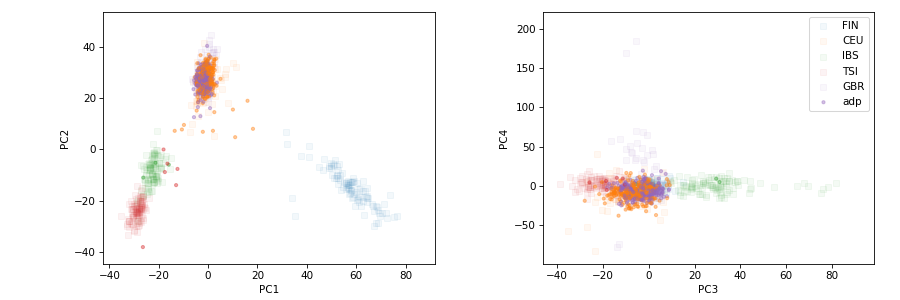
\includegraphics[width=0.98\textwidth]{img/ukb_snpscap_kgn_bial_orphans_5c_pred_EUR_sturef_kgn_bial_orphans_snps_ukb_snpscap_ukb_EUR_adp}
  \caption{PC scores of the European in the 500 randomly selected global samples UK Biobank data (circles) predicted by the four methods with the European samples in the 1000 Genomes data (squares) as the reference.}
\end{figure}

\begin{figure}[p]
  \centering
  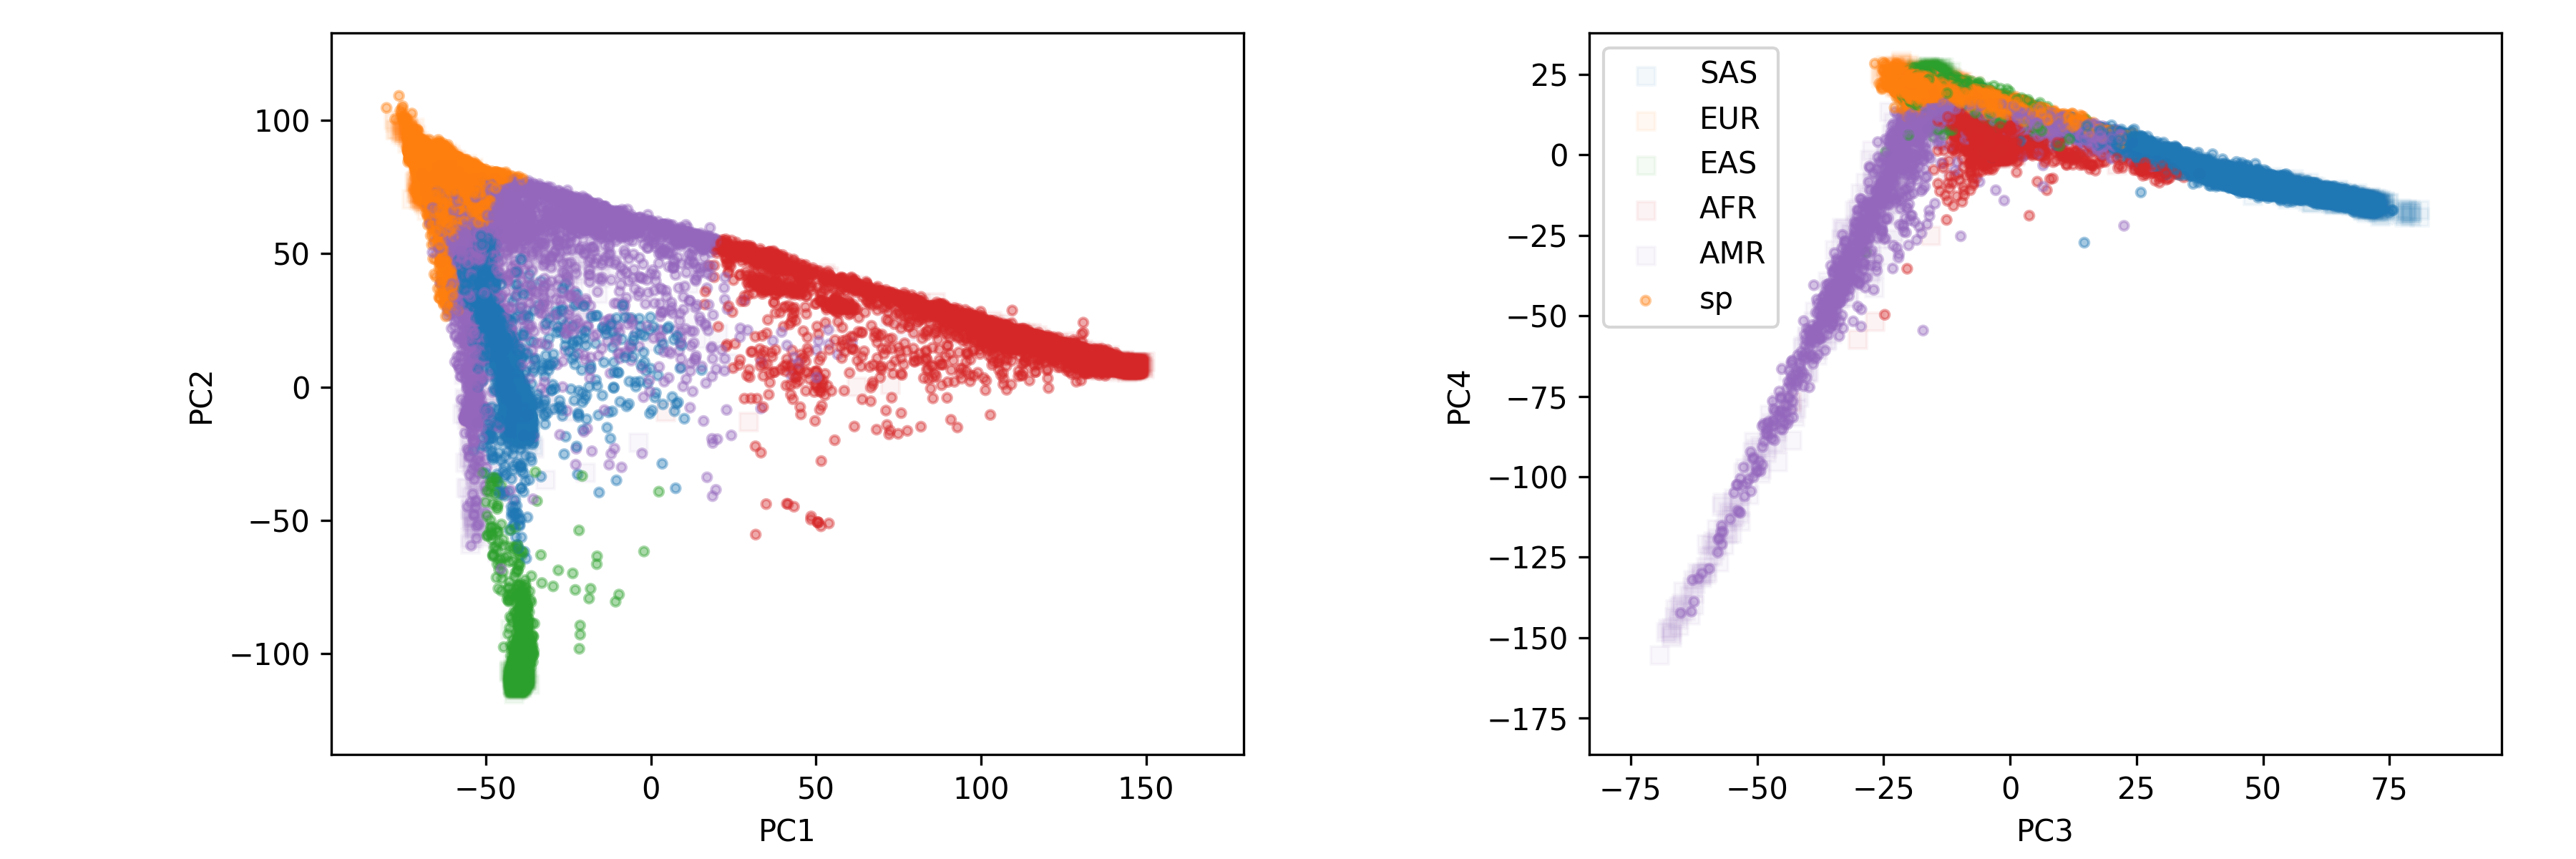
\includegraphics[width=0.98\textwidth]{img/ukb_snpscap_kgn_bial_orphans_nchunks100_sturef_kgn_bial_orphans_snps_ukb_snpscap_ukb_sp.png}
  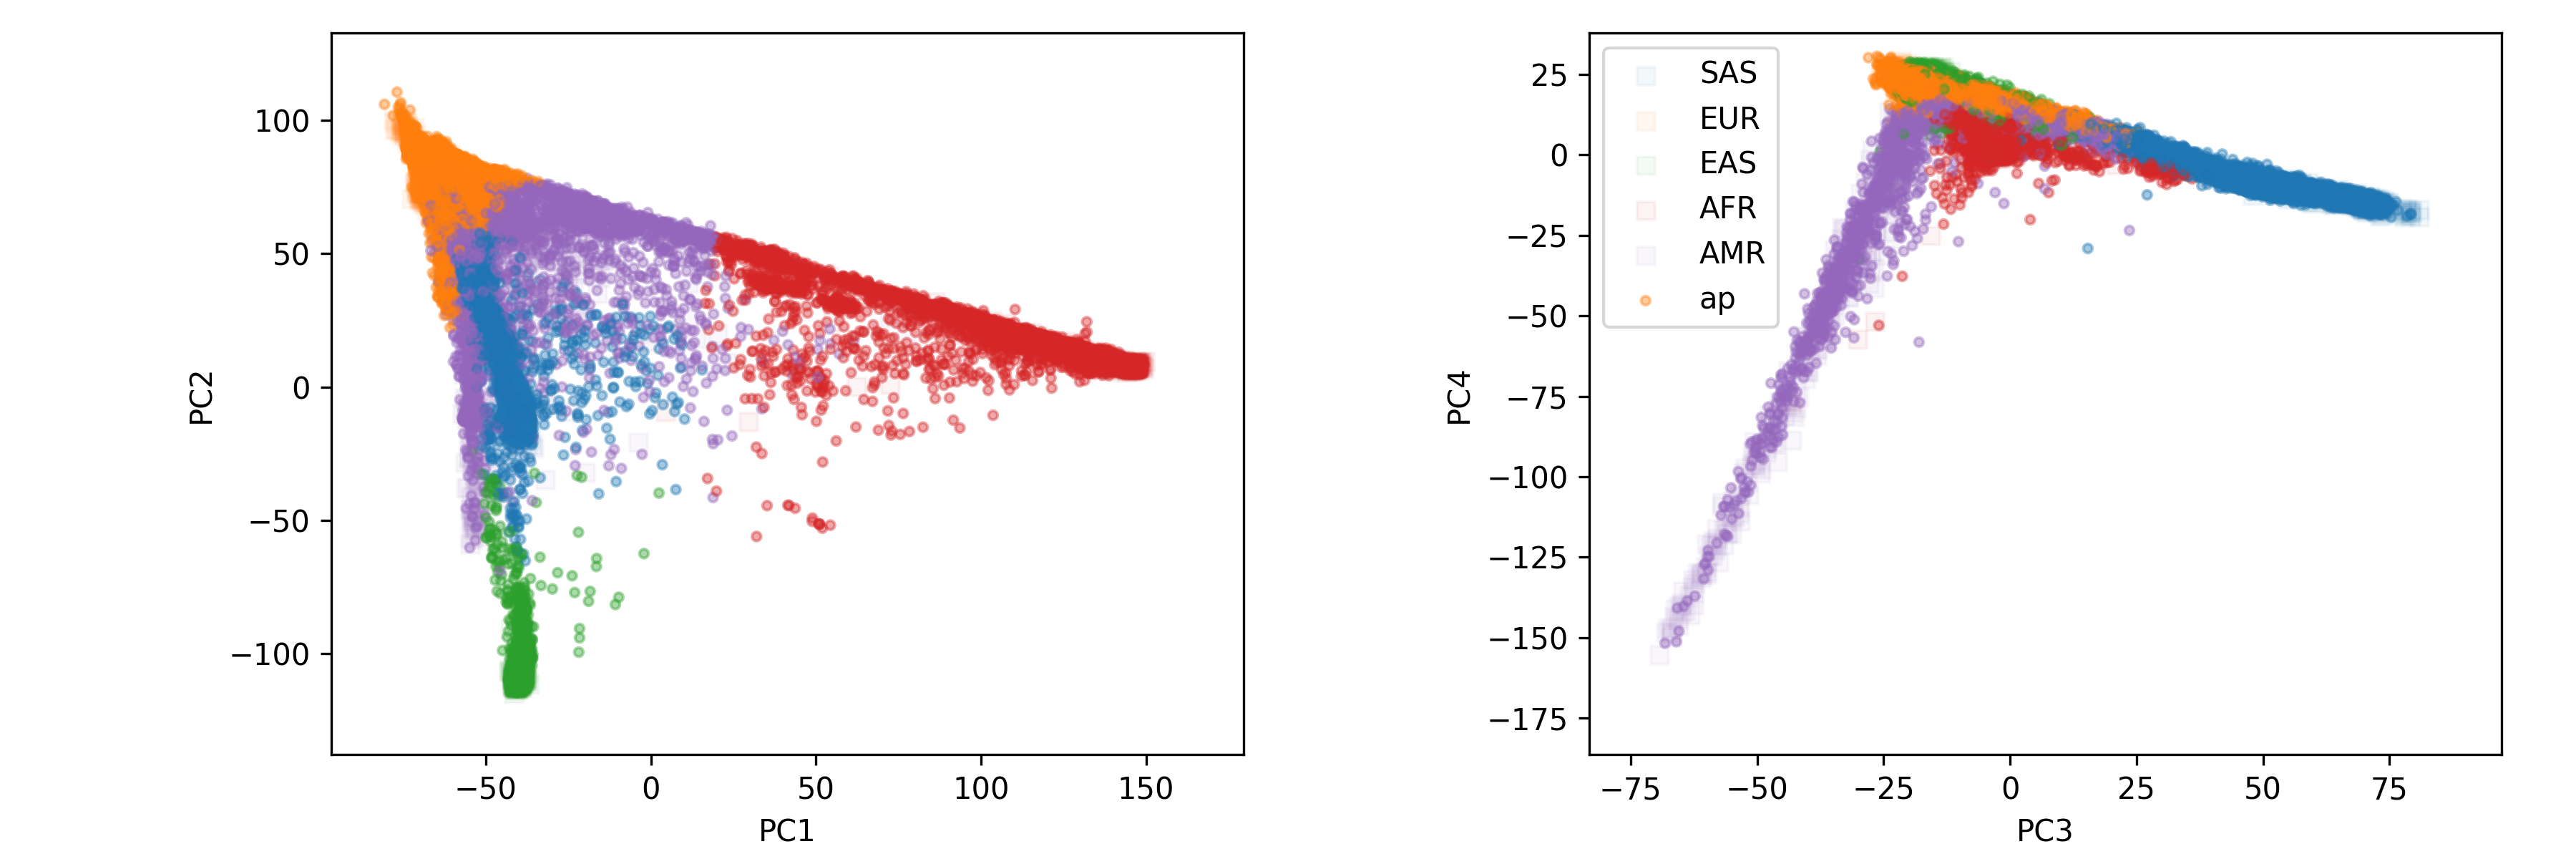
\includegraphics[width=0.98\textwidth]{img/ukb_snpscap_kgn_bial_orphans_nchunks100_sturef_kgn_bial_orphans_snps_ukb_snpscap_ukb_ap.png}
  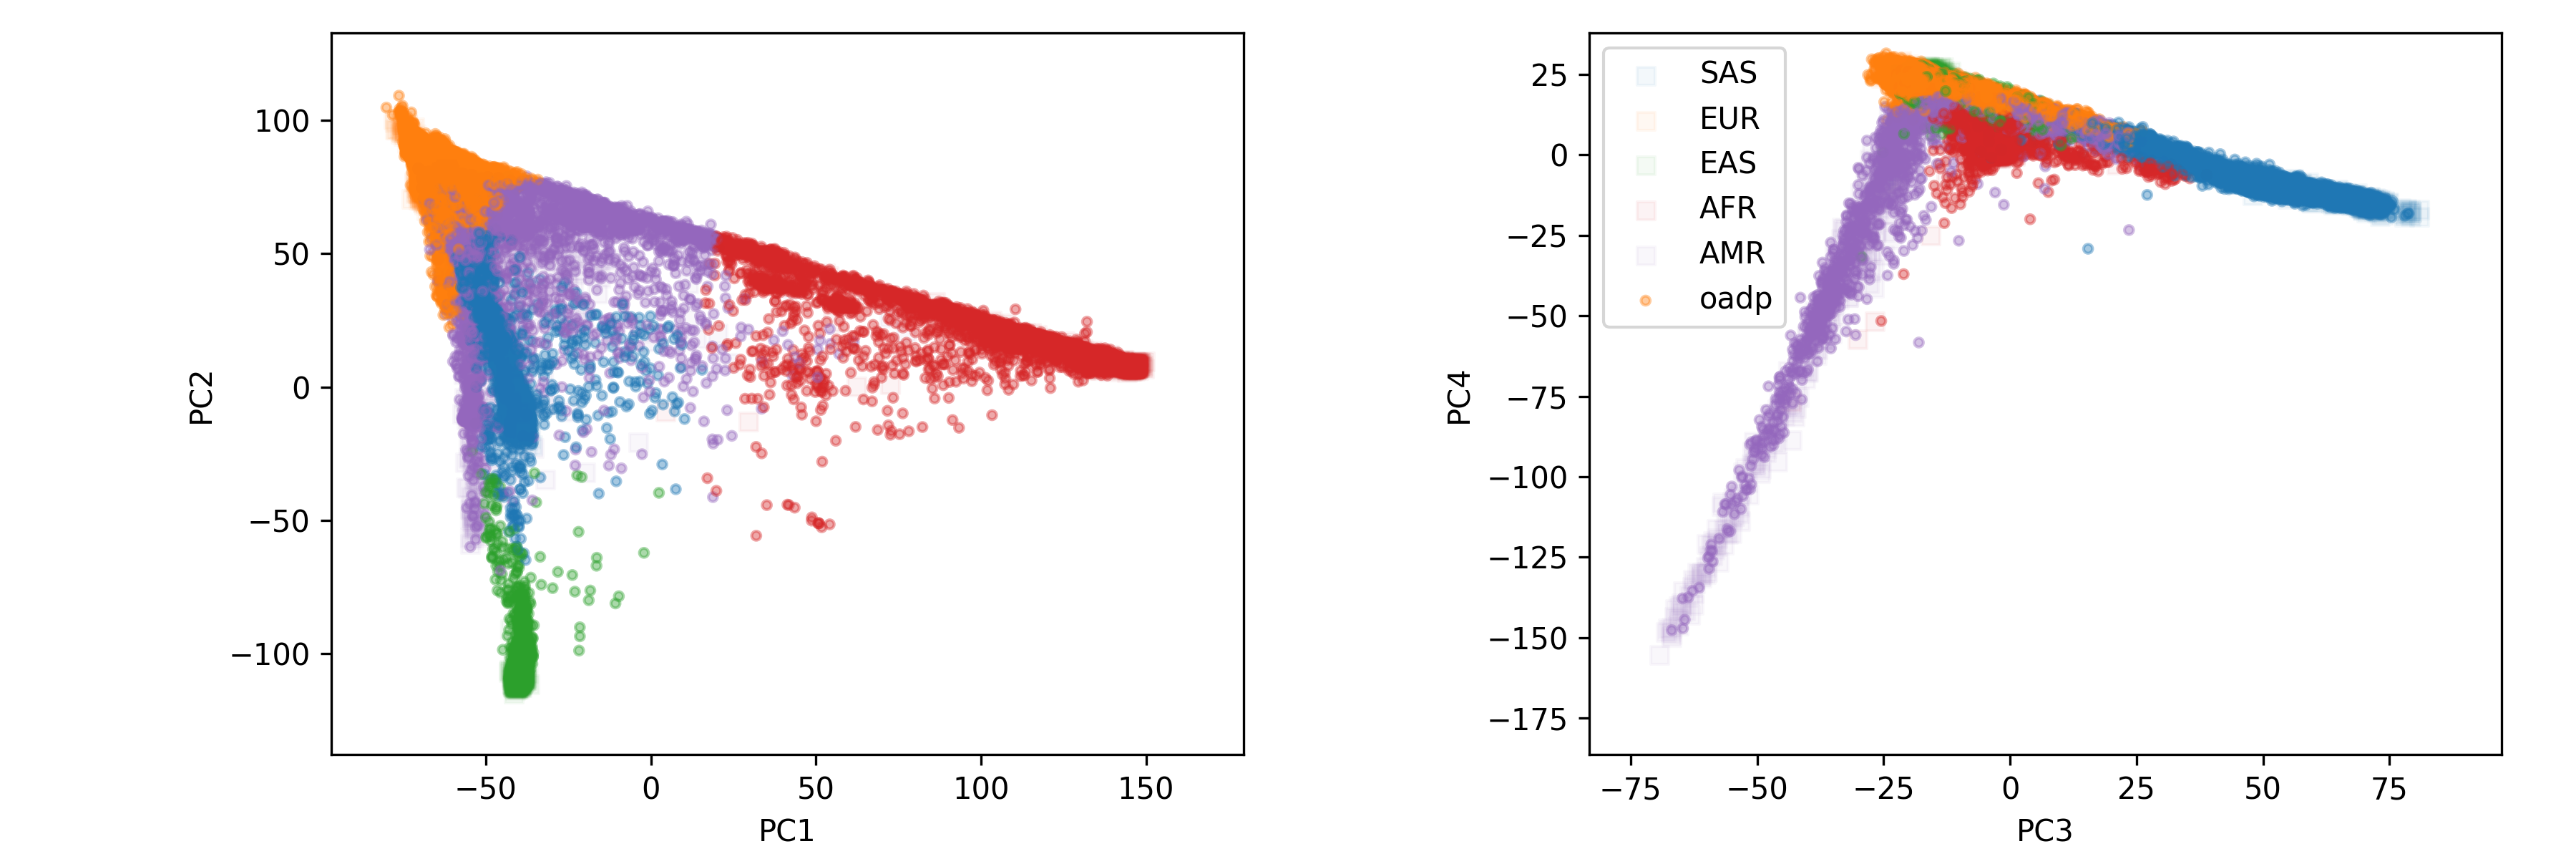
\includegraphics[width=0.98\textwidth]{img/ukb_snpscap_kgn_bial_orphans_nchunks100_sturef_kgn_bial_orphans_snps_ukb_snpscap_ukb_oadp.png}
  \caption{All the 488366 samples in the UK Biobank data.}
\end{figure}

\begin{figure}[p]
  \centering
  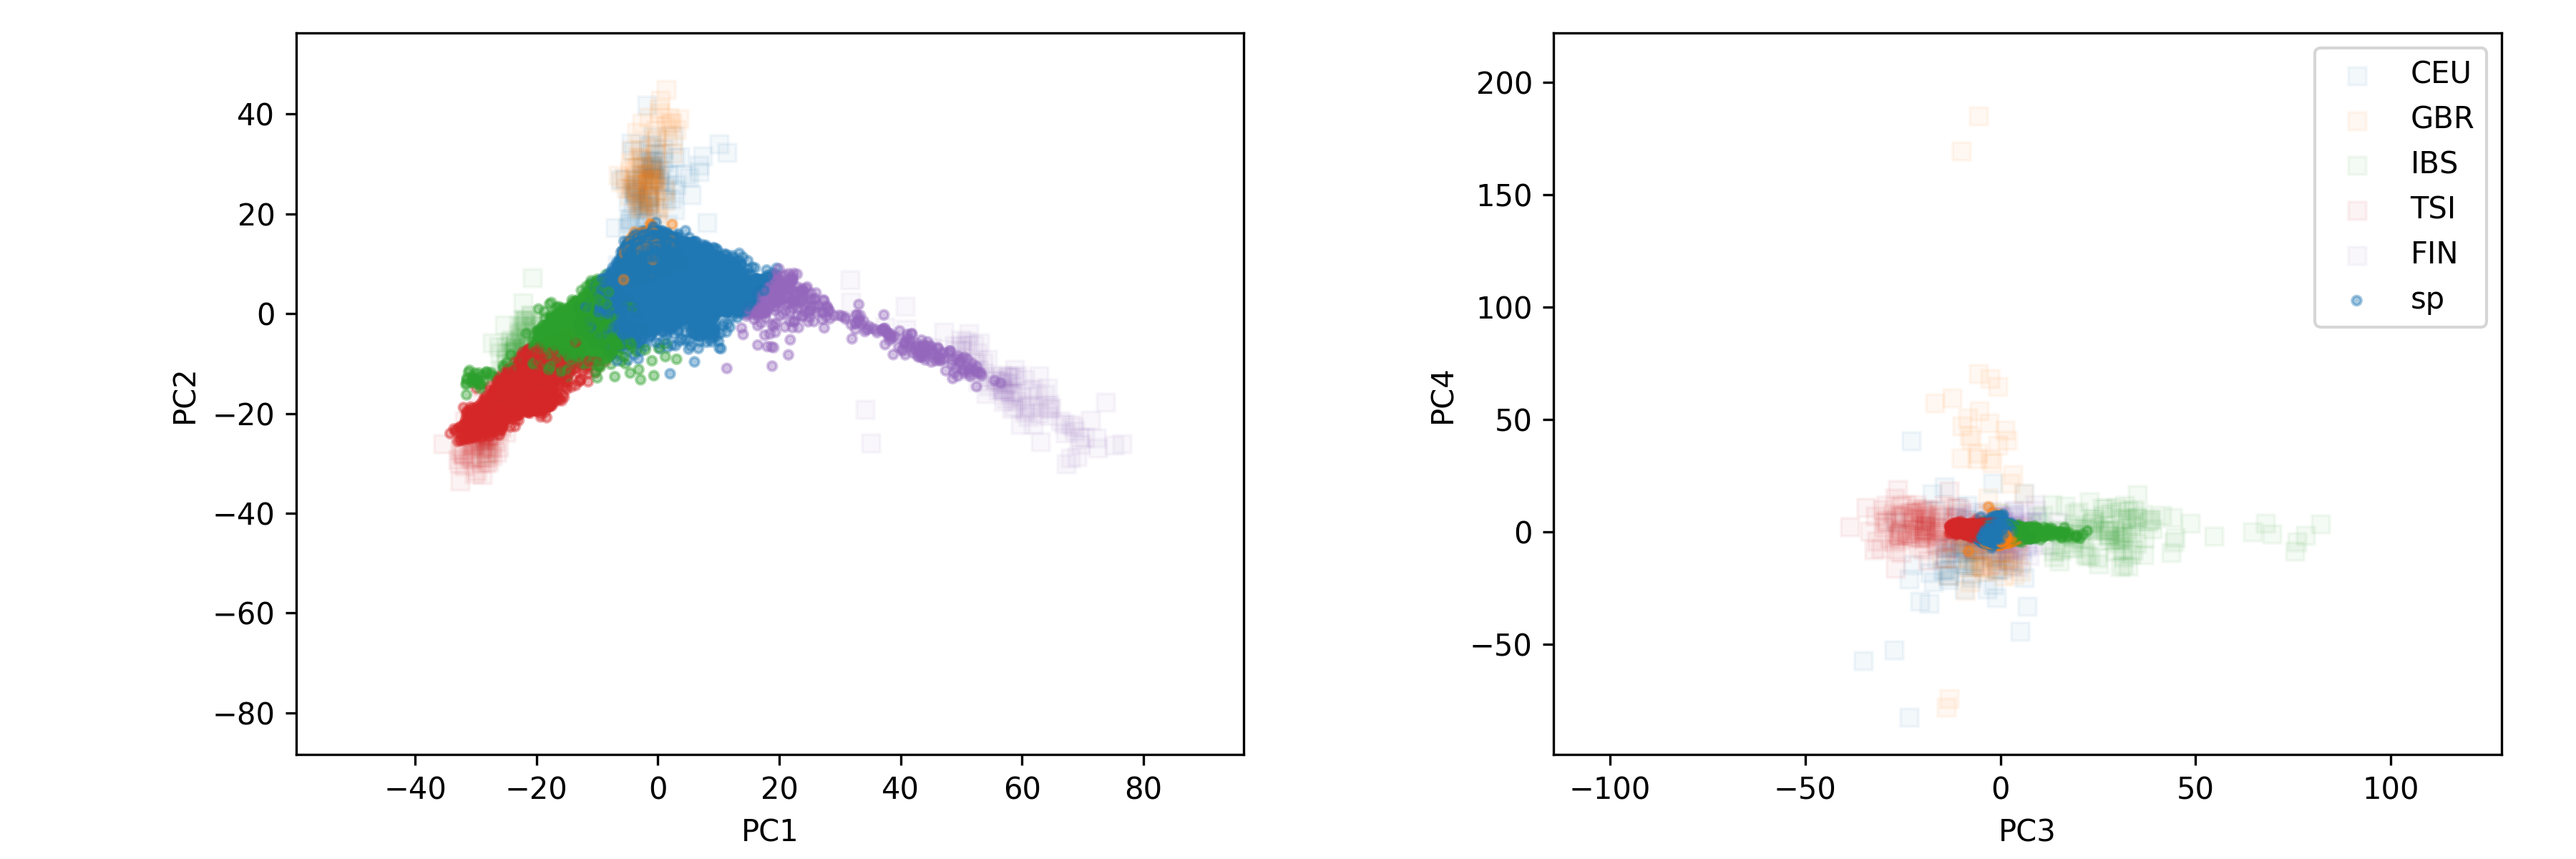
\includegraphics[width=0.98\textwidth]{img/ukb_snpscap_kgn_bial_orphans_pred_EUR_nchunks100_sturef_kgn_bial_orphans_snps_ukb_snpscap_ukb_EUR_sp.png}
  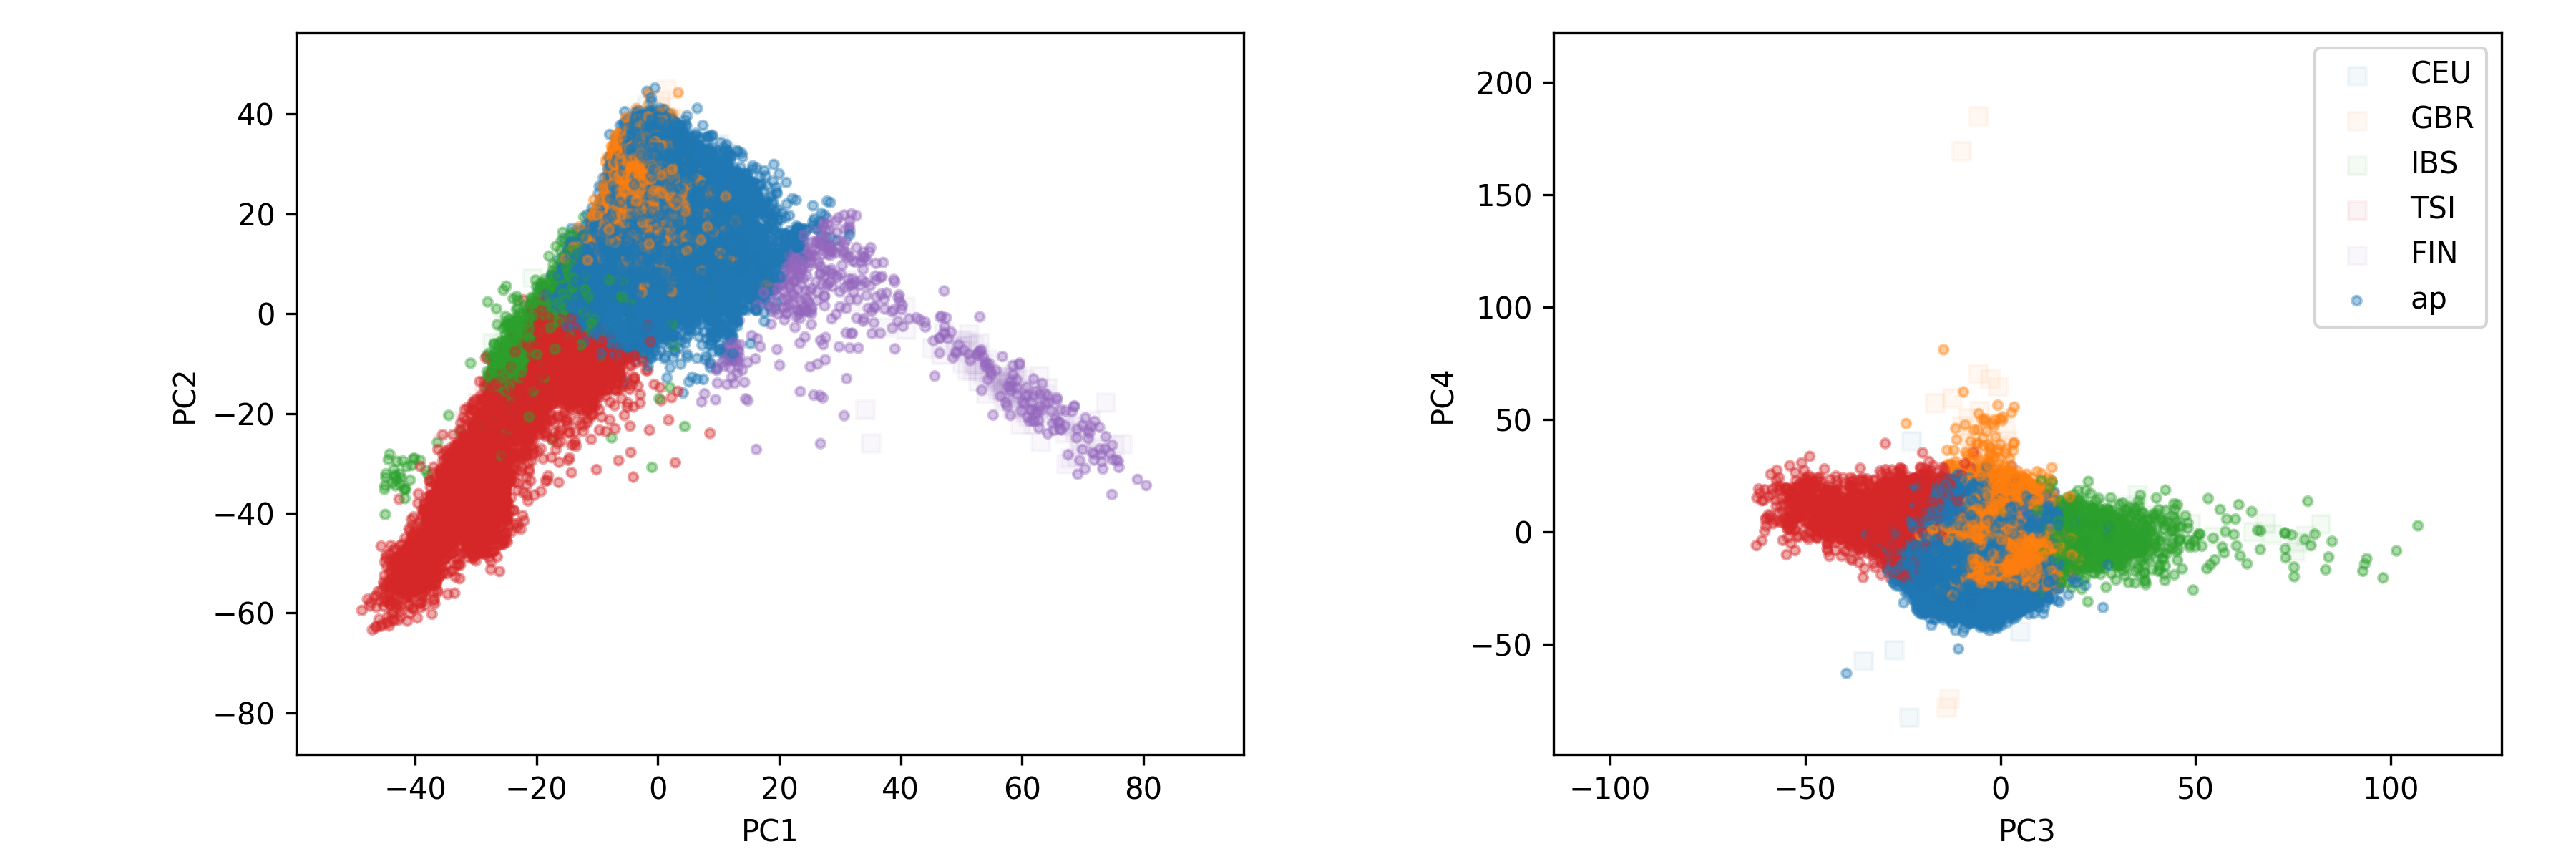
\includegraphics[width=0.98\textwidth]{img/ukb_snpscap_kgn_bial_orphans_pred_EUR_nchunks100_sturef_kgn_bial_orphans_snps_ukb_snpscap_ukb_EUR_ap.png}
  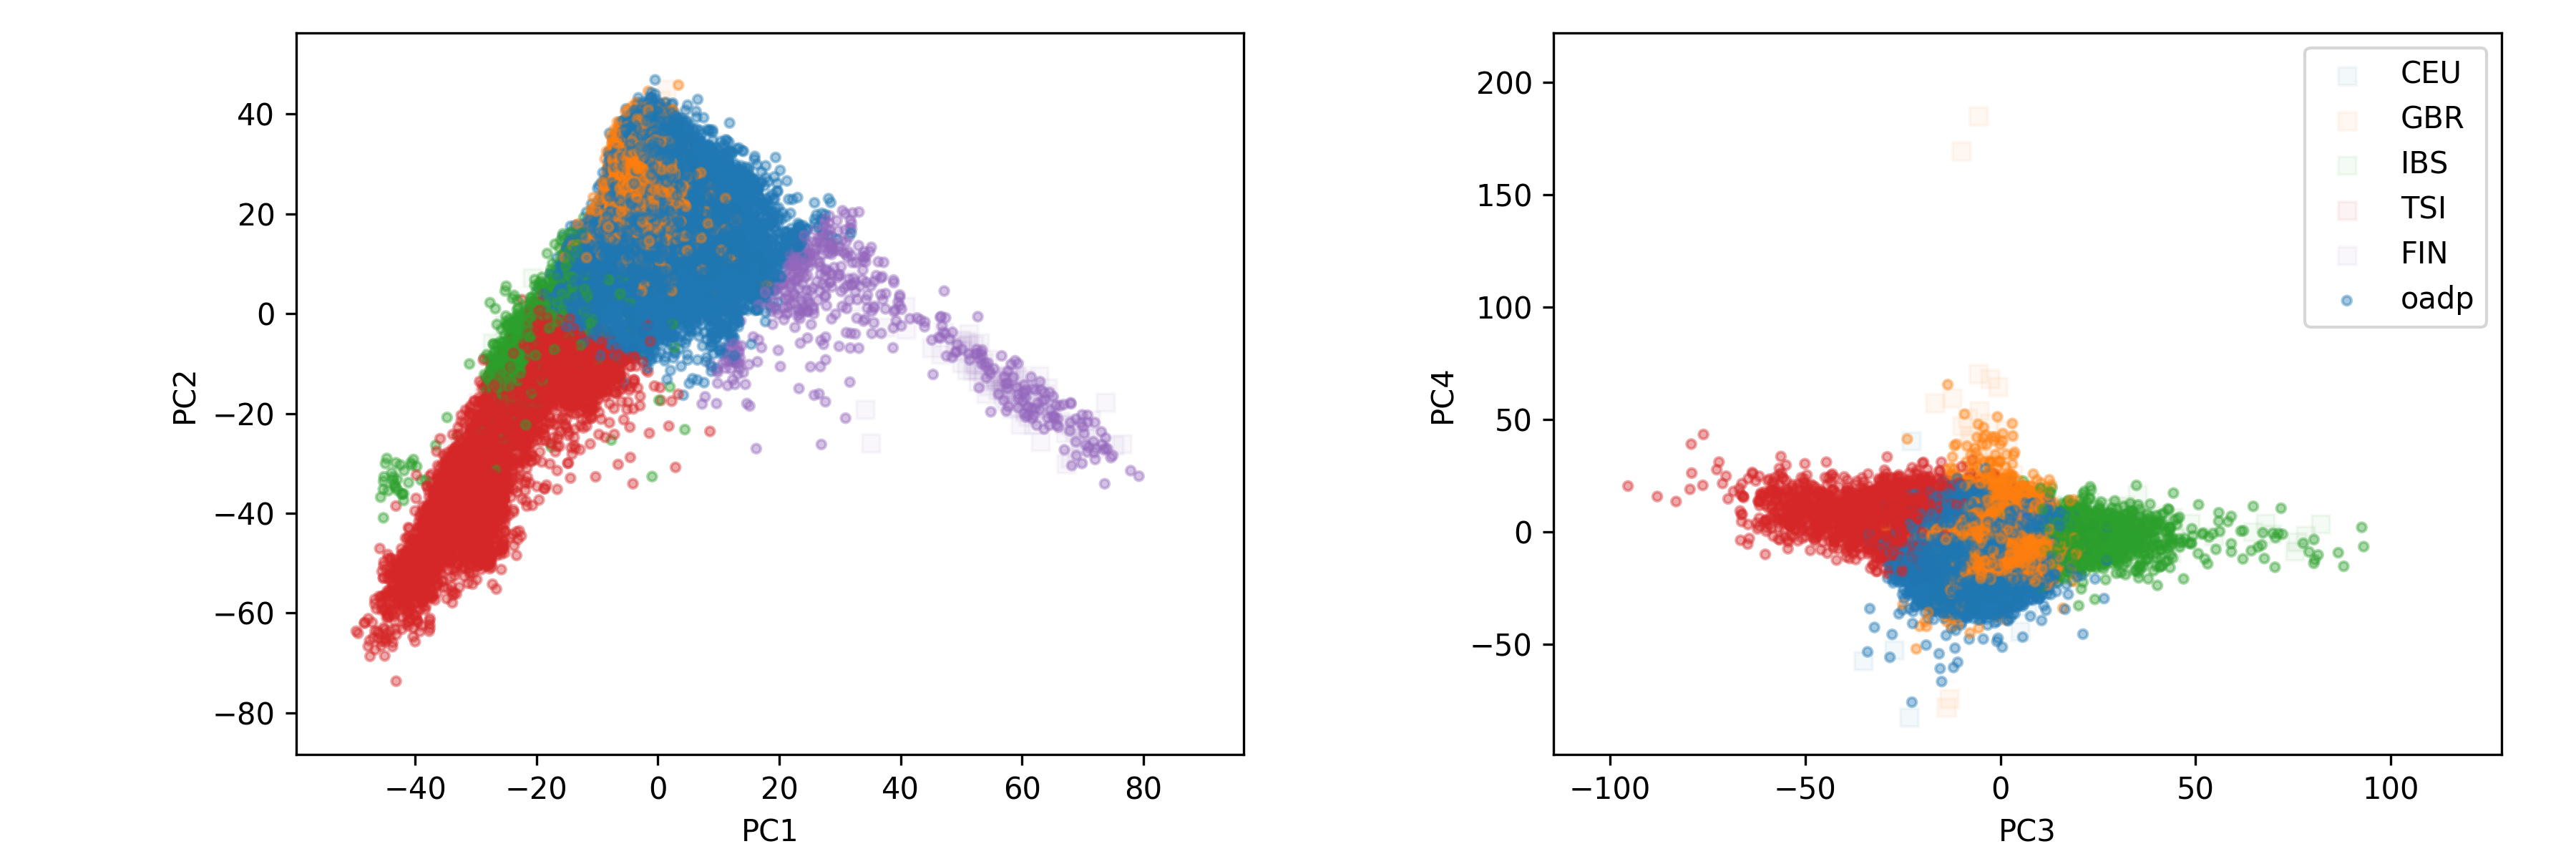
\includegraphics[width=0.98\textwidth]{img/ukb_snpscap_kgn_bial_orphans_pred_EUR_nchunks100_sturef_kgn_bial_orphans_snps_ukb_snpscap_ukb_EUR_oadp.png}
  \caption{All the 462284 European samples in the UK Biobank data.}
\end{figure}


\end{document}

% \begin{figure}[p]
%   \centering
%   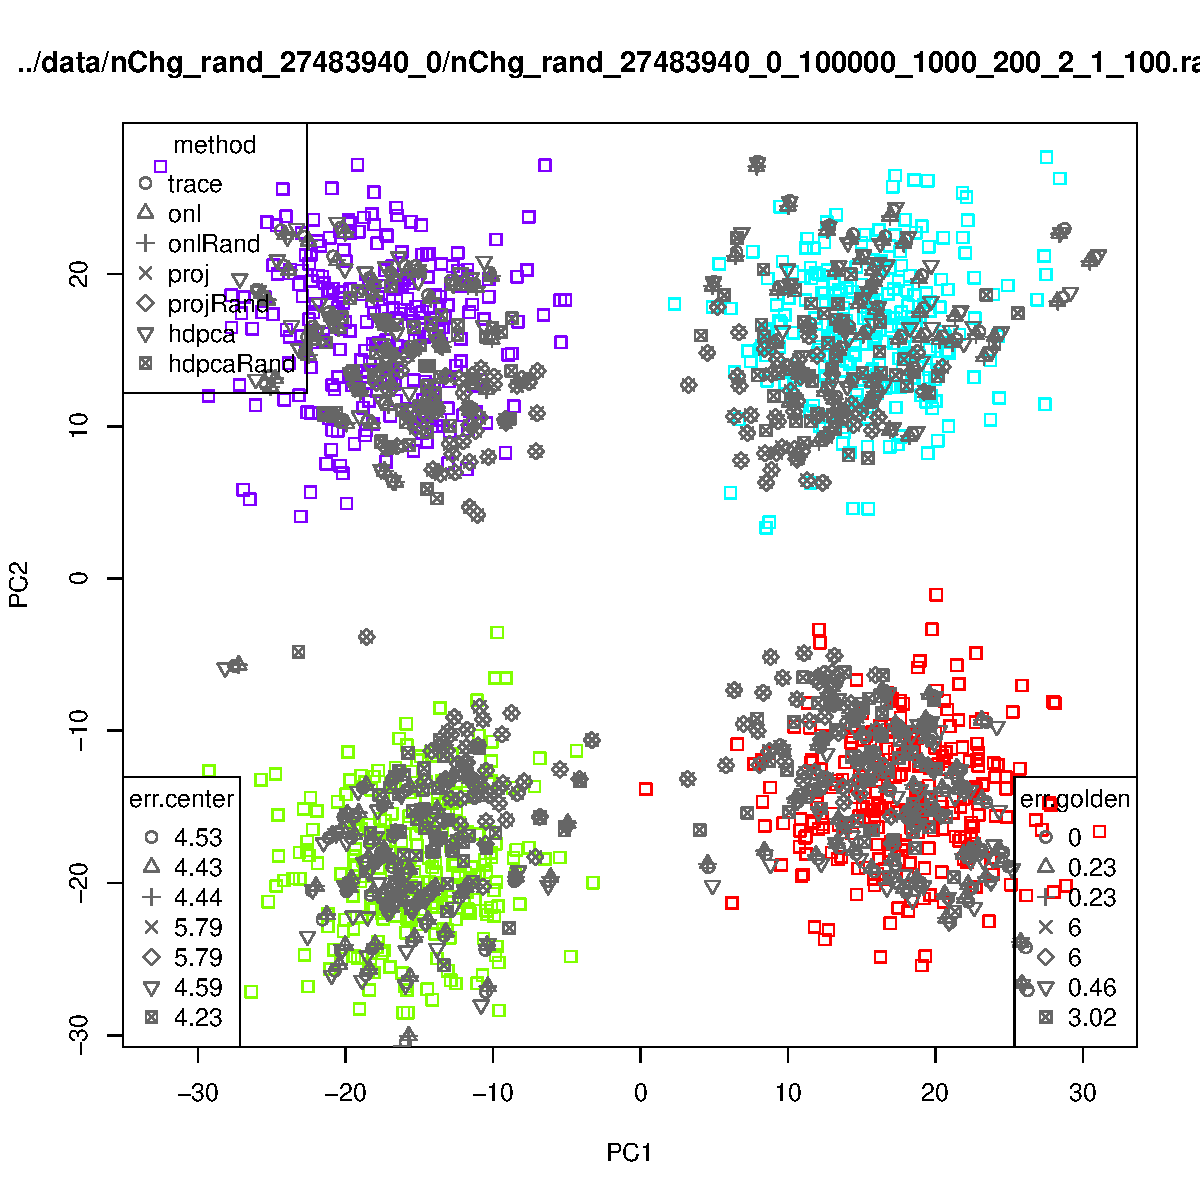
\includegraphics[width=0.98\textwidth]{n1000}
%   \caption{
%     Predicted PC scores on top of reference PC scores.
%     The four populations in the $2 \times 2$ grid simulated by the GGS software can be clearly identified.
%     Reference individuals are in color,
%     while predicted PC scores for the study individuals are in gray.
%     Two measurements of deviations (accuracy) are used.
%     The reference center error is the square root of the average squared distance between the study individuals and the population centers, which are the means of the PC scores of the reference individuals by the populations.
%     The golden standard error is the square root of the averate squared distance between the study individuals' PC scores predicted by different methods compared to the golden standard result, which in our case is the PC scores predicted by ADP.
%     The reference size is 1000 and the study size is 200.
%     There are 100,000 loci (1000 per genealogy) and the migration rate is 100.
%   }
%   \label{fig:n1000}
% \end{figure}

% \begin{figure}[p]
%   \centering
%   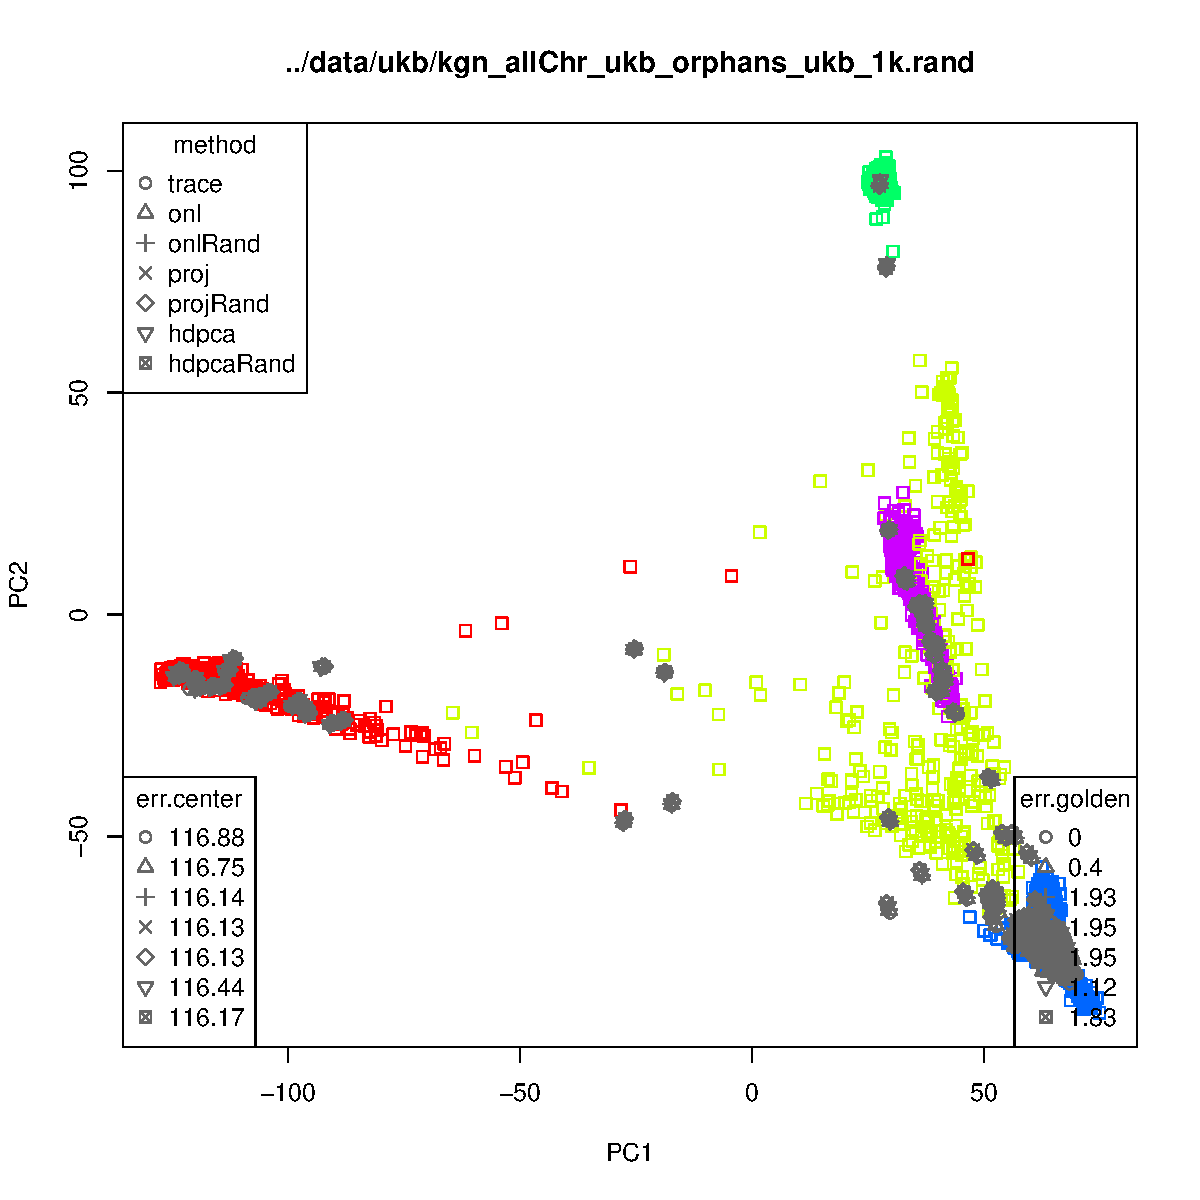
\includegraphics[width=0.98\textwidth]{ukb}
%   \caption{
%     The reference individuals are from the 1000 Genomes dataset with 2492 unrelated individuals from 5 superpopulations: African, American, East Asian, European, and South Asian. 
%     The study sample contain 1000 individuals from the UKBioBank dataset.
%     There are about 125,000 loci shared by the reference and study data.
%     The golden standard error is the square root of the averate squared distance between the study individuals' PC scores predicted by different methods compared to the golden standard result, which in our case is the PC scores predicted by ADP.
%   }
%   \label{fig:ukb}
% \end{figure}

% \begin{figure}[p]
%   \centering
%   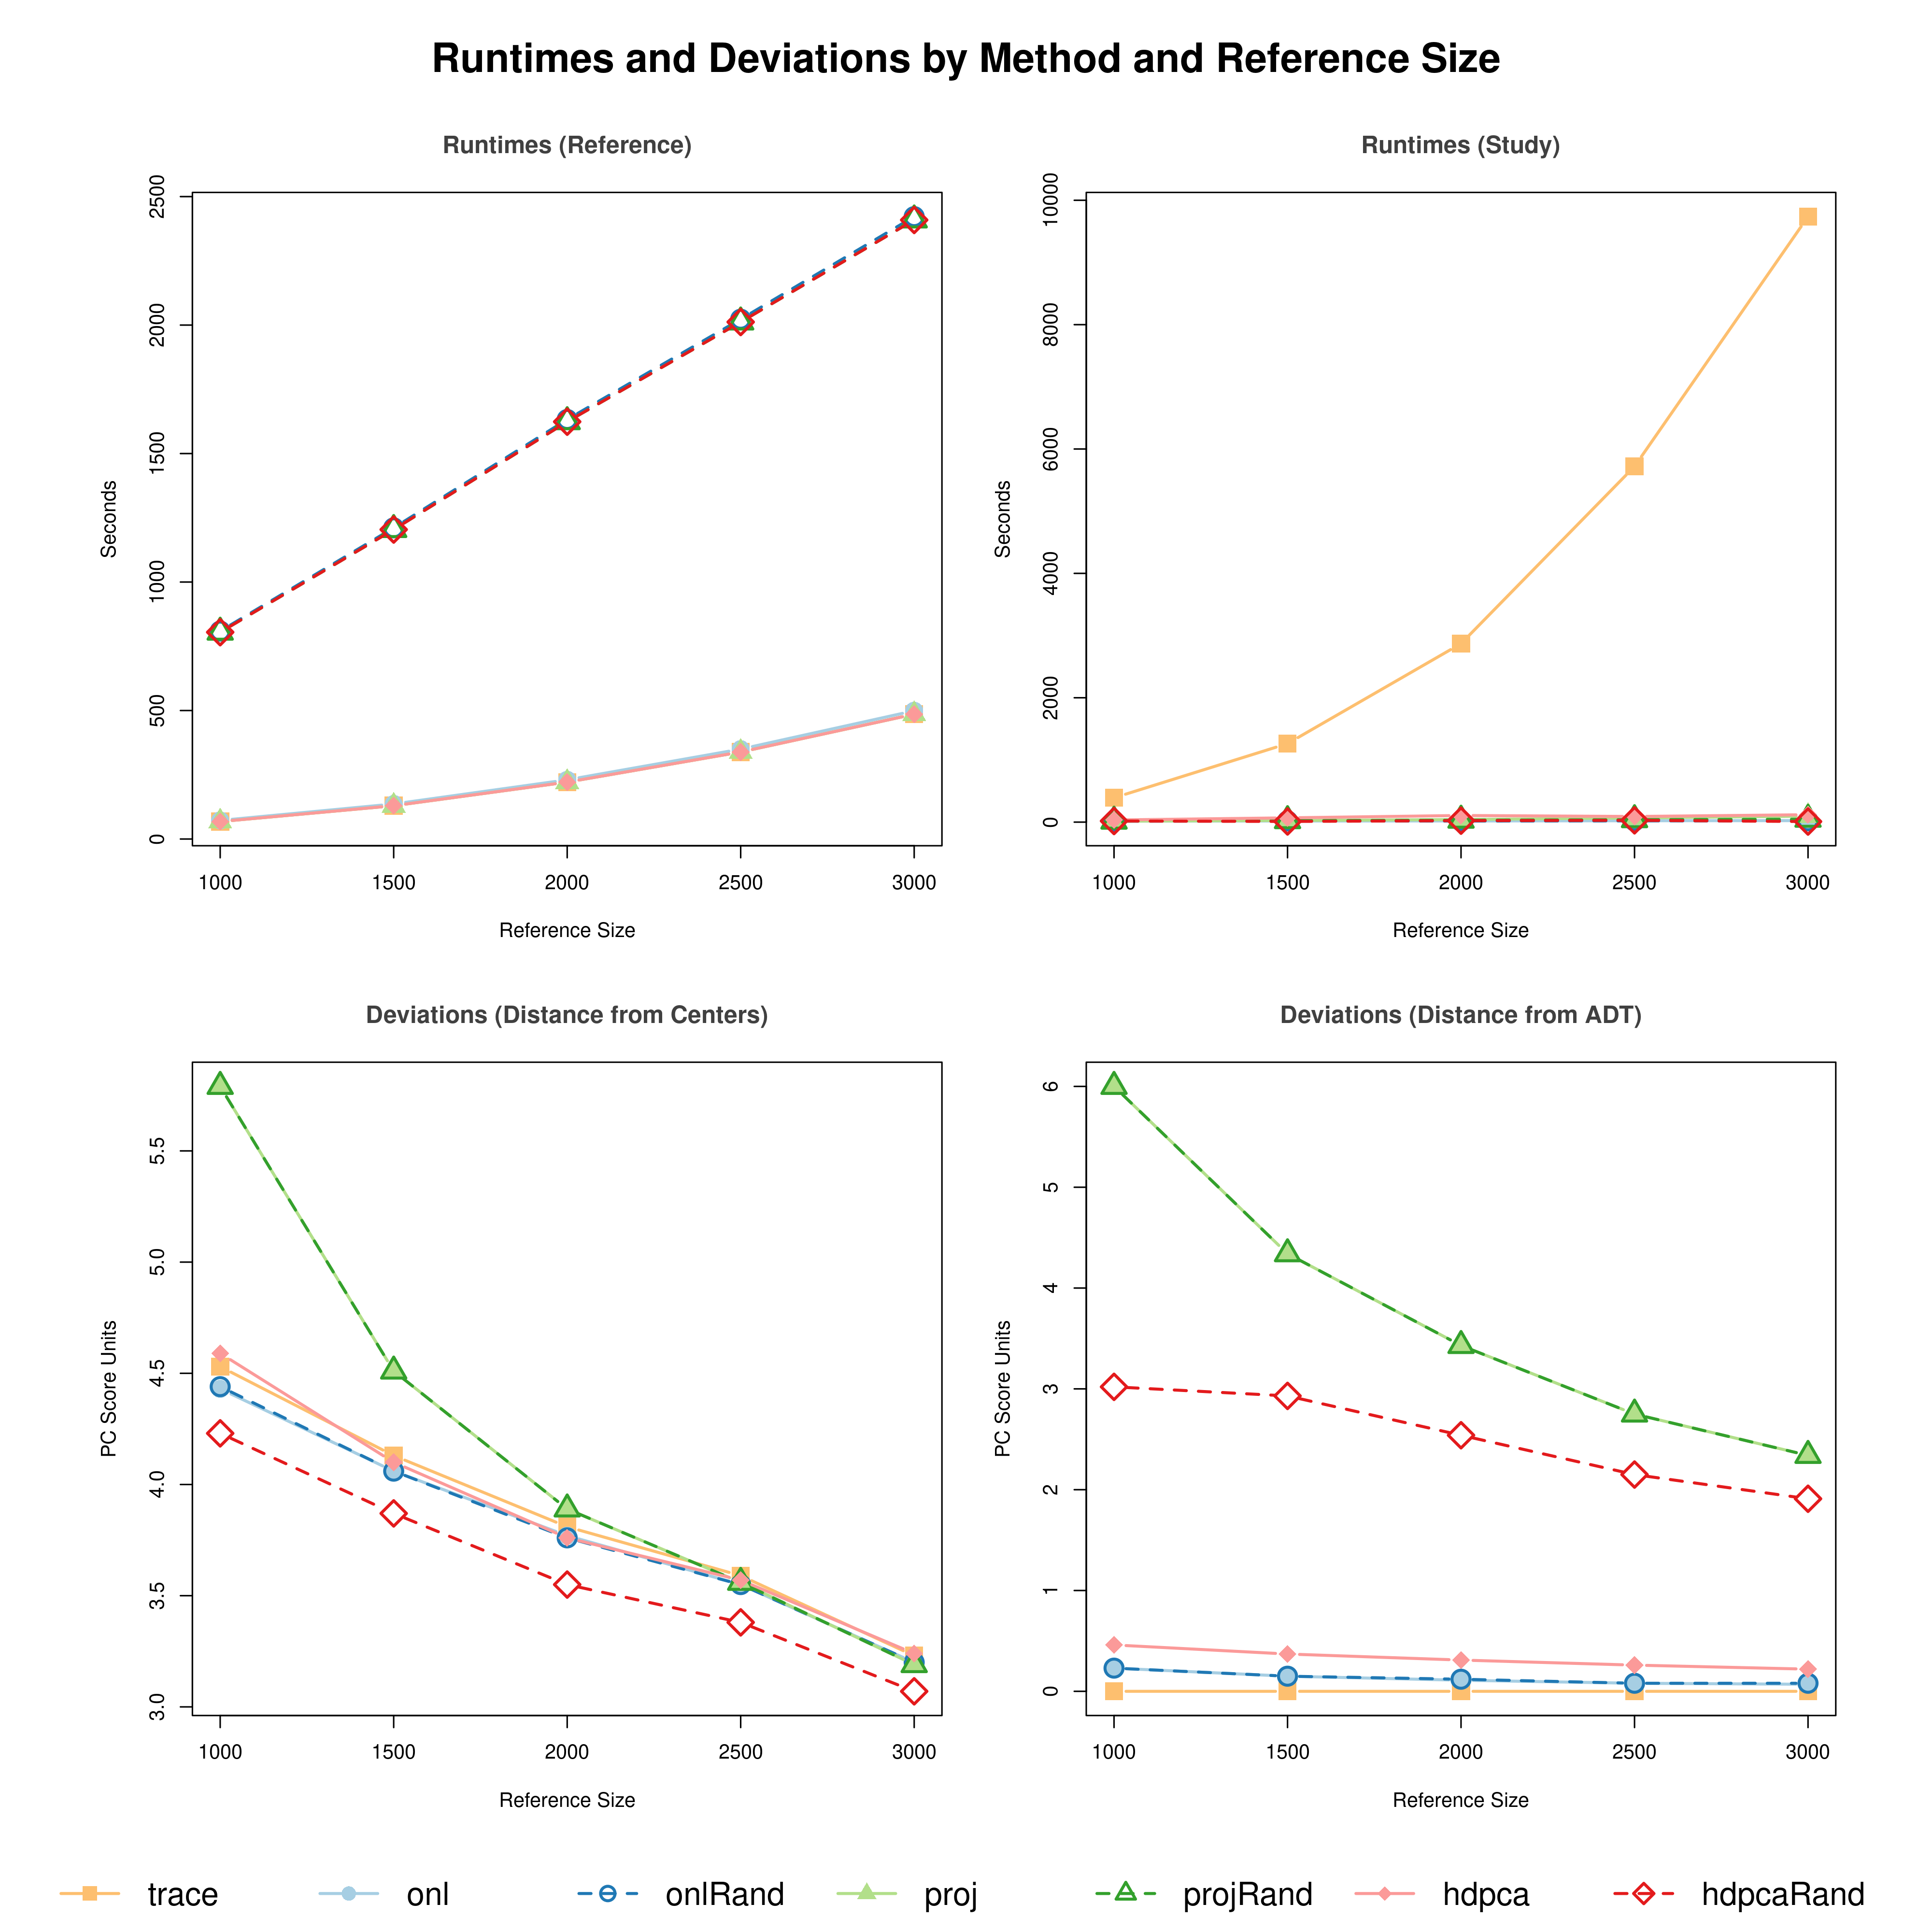
\includegraphics[width=0.98\textwidth]{img/nChg}
%   \caption{
%     Runtimes and deviations for different methods as the reference sample size increases.
%     The study size is fixed to 200 and the number of SNPs is 100,000 (1000 per genealogy). 
%     Simulation is done on a $2 \times 2$ grid with a migration rate of 100 by the GGS software. 
%   }
%   \label{fig:nChg}
% \end{figure}

% \begin{figure}[p]
%   \centering
%   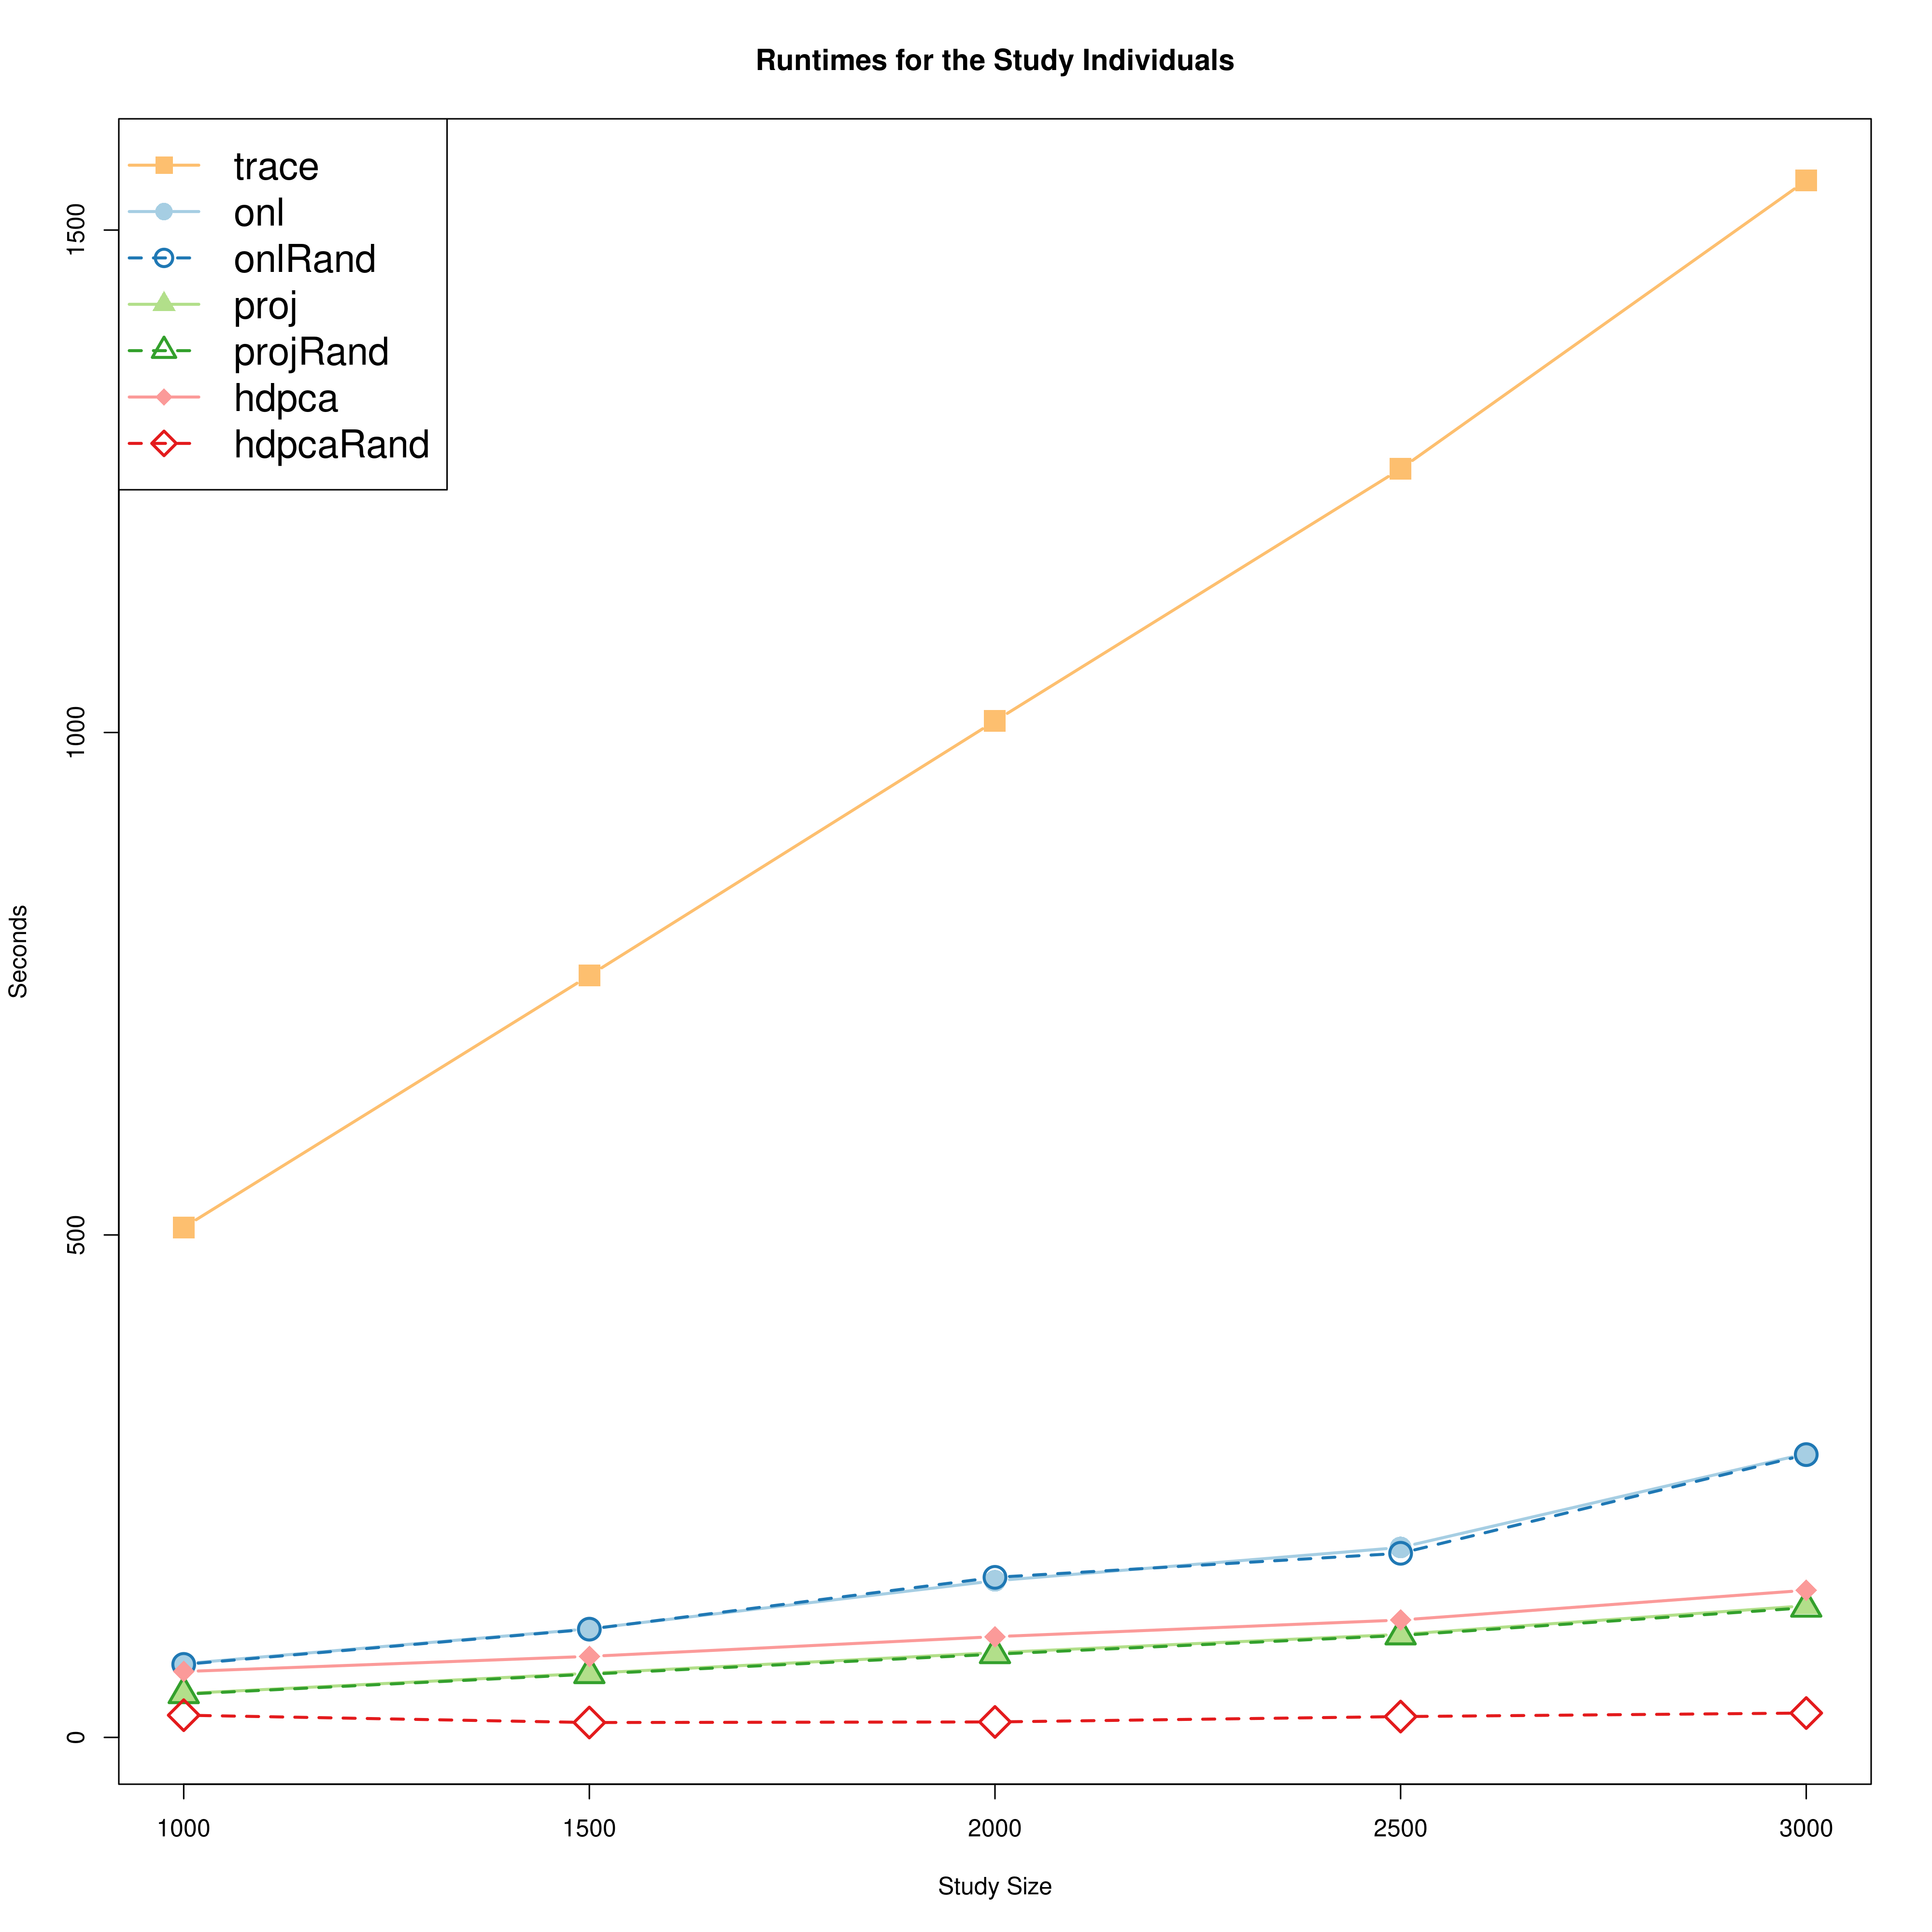
\includegraphics[width=0.98\textwidth]{img/mChg}
%   \caption{
%     Runtimes and deviations for different methods as the study sample size increases.
%     The reference sample size is fixed to 600 and the number of SNPs is 100,000 (1000 per genealogy).
%     Simulation is done on a $2 \times 2$ grid with a migration rate of 100 by the GGS software. 
%   }
%   \label{fig:mChg}
% \end{figure}

% \includegraphics[width=0.98\textwidth]{runtimes_rand}

% \includegraphics[width=0.98\textwidth]{err_refcenter_rand}

% \includegraphics[width=0.98\textwidth]{err_trace_rand}

% \includegraphics[width=0.98\textwidth]{err_refcenter_rand}

% \includegraphics[width=0.98\textwidth]{kgn_allChr_ukb_orphans_ukb_1k_comb}

% \includegraphics[width=0.98\textwidth]{kgn_allChr_ukb_orphans_ukb_1k_rand}

% \begin{table} 
%   \centering
%   \begin{tabular}{|l|l|l|l|l|}
%     \hline
%     Method & Reference Runtimes (n=2492) & Study Runtimes (m=1000)& Golden Standard Error \\ 
%     \hline
%     ADP & 411 & 29813 & 0.00 \\
%     \hline
%     OADP & 2518 & 103 & 0.40 \\
%     \hline
%     SP & 411 & 425 & 1.95 \\
%     \hline
%     AP & 411 & 482 & 1.12 \\
%     \hline
%   \end{tabular}
%   \caption{
%     Comparison of runtimes and accuracy for different methods applied to the real-life datasets.
%     The reference individuals are from the 1000 Genomes dataset with 2492 unrelated individuals.
%     The study sample contain 1000 individuals from the UKBioBank dataset.
%     There are about 125,000 loci shared by the reference and study data.
%     The golden standard error is the square root of the averate squared distance between the study individuals' PC scores predicted by different methods compared to the golden standard result, which in our case is the PC scores predicted by ADP.
%   }
%   \label{tbl:ukb}
% \end{table} 

% \begin{table}
%   \centering
%   \begin{tabular}{|l|l|l|l|l|l|}
%     \hline
%     Reference Size & 1000 & 1500 & 2000 & 2500 & 3000 \\
%     \hline
%     ADP        &  68  & 1263 & 2871 & 5720 & 9737 \\
%     OADP       &  72  & 18   & 19   & 22   & 24   \\
%     SP         &  68  & 26   & 42   & 67   & 96   \\
%     AP         &  68  & 69   & 107  & 91   & 119  \\
%     \hline
%   \end{tabular}
%   \caption{
%     Reference runtimes for the simulated data as the reference size increases.
%     The study size is fixed to 200 and the number of SNPs is 100,000 (1000 per genealogy). 
%     Simulation is done on a $2 \times 2$ grid with a migration rate of 100 by the GGS software. 
%   }
%   \label{tbl:nChg-runtimes-ref}
% \end{table}

% \begin{table}
%   \centering
%   \begin{tabular}{|l|l|l|l|l|l|}
%     \hline
%     Reference Size & 1000 & 1500 & 2000 & 2500 & 3000 \\
%     \hline
%     ADP        & 391  &  130 &  222 &  339 &  486 \\
%     OADP       & 15   &  136 &  230 &  350 &  499 \\
%     SP         & 16   &  130 &  222 &  339 &  486 \\
%     AP         & 34   &  130 &  222 &  339 &  486 \\
%     \hline
%   \end{tabular}
%   \caption{
%     Study runtimes for simulated data as the reference size increases.
%     The study size is fixed to 200 and the number of SNPs is 100,000 (1000 per genealogy). 
%     Simulation is done on a $2 \times 2$ grid with a migration rate of 100 by the GGS software. 
%   }
%   \label{tbl:nChg-runtimes-study}
% \end{table}

% \begin{table}
%   \centering
%   \begin{tabular}{|l|l|l|l|l|l|}
%     \hline
%     Study Size & 1000  & 1500 & 2000 & 2500 & 3000 \\
%     \hline
%     ADP        & 0.00  & 0.00 & 0.00 & 0.00 & 0.00 \\
%     OADP       & 0.23  & 0.15 & 0.11 & 0.08 & 0.07 \\
%     SP         & 6.00  & 4.34 & 3.43 & 2.75 & 2.34 \\
%     AP         & 0.46  & 0.37 & 0.31 & 0.26 & 0.22 \\
%     \hline
%   \end{tabular}
%   \caption{
%     Golden standard error for the simulated data as the reference size increases.
%     The study size is fixed to 200 and the number of SNPs is 100,000 (1000 per genealogy). 
%     Simulation is done on a $2 \times 2$ grid with a migration rate of 100 by the GGS software. 
%   }
%   \label{tbl:nChg-accuracy-gold}
% \end{table}

% \begin{table}
%   \centering
%   \begin{tabular}{|l|l|l|l|l|l|}
%     \hline
%     Reference Size & 1000  & 1500 & 2000 & 2500 & 3000 \\
%     \hline
%     ADP        & 4.53  & 4.13 & 3.81 & 3.59 & 3.23 \\
%     OADP       & 4.43  & 4.06 & 3.77 & 3.55 & 3.20 \\
%     SP         & 5.79  & 4.51 & 3.89 & 3.56 & 3.19 \\
%     AP         & 4.59  & 4.10 & 3.76 & 3.57 & 3.24 \\
%     \hline
%   \end{tabular}
%   \caption{
%     Geographic center error for the simulated data as the reference size increases.
%     The study size is fixed to 200 and the number of SNPs is 100,000 (1000 per genealogy). 
%     Simulation is done on a $2 \times 2$ grid with a migration rate of 100 by the GGS software. 
%   }
%   \label{tbl:nChg-accuracy-ctr}
% \end{table}

% \begin{table}
%   \centering
%   \begin{tabular}{|l|l|l|l|l|l|}
%     \hline
%     Reference Size & 1000 & 1500 & 2000 & 2500 & 3000 \\
%     \hline
%     ADP        & 507  & 758 & 1011 & 1262 & 1549 \\
%     OADP       &  73  & 108 &  156 &  189 &  282 \\
%     SP         &  44  &  64 &   84 &  103 &  131 \\
%     AP         &  66  &  81 &  100 &  117 &  146 \\
%     \hline
%   \end{tabular}
%   \caption{
%     Study runtimes for the simulated data as the study size increases.
%     The reference size is fixed to 600 and the number of SNPs is 100,000 (1000 per genealogy). 
%     Simulation is done on a $2 \times 2$ grid with a migration rate of 100 by the GGS software. 
%   }
%   \label{tbl:mChg-runtimes-study}
% \end{table}


% \section{Randomized SVD}\label{sec:randsvd}

% In addition to estimating the PC scores of the study individuals,
% we have another algorithm that aims at improving the decomposition of the
% training data.
% For SP, AP, ADP, and OADP, we need to find the covariance matrix of the training
% data, which has dimension $n \times n$, and conduct eigendecomosition on it.
% However, when $n$ is exceedingly large,
% computation and memory cost of PCA on the reference samples can be enormous.
% A randomized SVD (RSVD) algorithm has been developed to handle this issue.
% When the reference sample size is small, RSVD can be slower than standard SVD,
% but it is scalable to large sample size.
% For the details of the RSVD algorithm, see \citet{halko2011finding}.

% Notice that the randomized SVD method on the training data
% only calculates the first $k$ eigenvalues.
% However, in order to use adjusted projection,
% all the eigenvalues of the training data are required.
% Thus for the missing eigenvalues,
% we predict them by regressing their log-scale values on the ranks
% and using the first $k$ eigenvalues for training the linear regression.
